\documentclass[11pt,a4paper]{article}
\usepackage[paperwidth=13.333in,paperheight=7.5in,margin=0pt]{geometry}

\usepackage[utf8]{inputenc}
\usepackage[T1]{fontenc}
\usepackage{lmodern}
\usepackage{amsmath,amssymb,amsfonts,bm}
\usepackage{graphicx}
\graphicspath{{../img/}{./img/}{img/}}
\usepackage{xcolor}
\usepackage{tikz}
\usetikzlibrary{calc,shapes.geometric,positioning}
\usepackage{booktabs}
\usepackage{array}
\usepackage{hyperref}

% Color Palette
\definecolor{navy}{HTML}{002060}
\definecolor{primaryblue}{HTML}{184C78}
\definecolor{accent}{HTML}{2980B9}
\definecolor{darkgray}{HTML}{2C3E50}
\definecolor{lightbg}{HTML}{F5F7FA}
\definecolor{bordergray}{HTML}{C8CDD2}
\definecolor{mutedgray}{HTML}{7F8C8D}
\definecolor{crimson}{HTML}{9E1636}
\definecolor{tunablered}{HTML}{C0392B}
\definecolor{gold}{HTML}{B48C14}
\definecolor{successgreen}{HTML}{27AE60}

\pagestyle{empty}
\setlength{\parindent}{0pt}

% Total Slides Count
\newcommand{\totalslides}{35}

% Positioning helper
\newcommand{\at}[4]{%
  \node[anchor=north west,inner sep=0pt,text width=#3in,align=left]
    at ([xshift=#1in,yshift=-#2in]current page.north west) {#4\par};}

% Per-slide line spacing (set at the start of a slide; tuned so the text fills its card)
\newcommand{\slidespread}[1]{\linespread{#1}\selectfont}

\newcommand{\fs}[2]{\fontsize{#1pt}{#2pt}\selectfont}

% Slide Header Macro: KU logo on top left, vertically aligned with blue column bar & title
\newcommand{\slideheader}[3]{%
  % Top-left KU Logo: width=0.70in, height=0.82in, vertically centered at y = -0.70in
  \node[anchor=west,inner sep=0pt]
    at ([xshift=0.50in,yshift=-0.70in]current page.north west)
    {
\includegraphics[width=0.70in,height=0.82in]{ku_logo.png}};
  % Vertical accent bar: left=1.35in, top=0.25in, height=0.90in -> vertical center = 0.70in
  \fill[accent] ([xshift=1.35in,yshift=-0.25in]current page.north west)
    rectangle ++(0.06in,-0.90in);
  % Title & Subtitle Node: vertically centered at y = -0.70in
  \node[anchor=west,inner sep=0pt,text width=11.2in,align=left]
    at ([xshift=1.55in,yshift=-0.70in]current page.north west) {%
      {\fs{11}{13}\bfseries\color{accent}\MakeUppercase{#1}\quad|\quad}%
      {\fs{20.5}{24}\bfseries\color{navy}#2}\\[0.18em]
      \if\relax\detokenize{#3}\relax\else{\fs{13}{16}\color{darkgray}#3}\fi
    };
}

% Slide Footer Macro
\newcommand{\slidefooter}[1]{%
  % Dividing Line
  \fill[bordergray] ([xshift=0.5in,yshift=-7.0in]current page.north west)
    rectangle ++(12.333in,-0.02in);
  % Left Date
  \at{0.5}{7.06}{2.5}{\fs{10}{12}\color{mutedgray}November 19, 2026}
  % Center Presenter Info
  \node[anchor=north,inner sep=0pt]
    at ([yshift=-7.06in]current page.north)
    {\fs{10}{12}\color{mutedgray}Chong Shik Park, Ph.D. \enspace$|$\enspace Korea University, Sejong \enspace$|$\enspace AI Applications in Accelerators};
  % Right Slide Number
  \node[anchor=north east,inner sep=0pt]
    at ([xshift=-0.5in,yshift=-7.06in]current page.north east)
    {\fs{10}{12}\bfseries\color{primaryblue}#1 / \totalslides};
}

% Standard Full-Width Content Card Macro
\newcommand{\drawcard}[5]{%
  \draw[rounded corners=8pt,fill=lightbg,draw=bordergray,line width=1.2pt]
    ([xshift=#1in,yshift=-#2in]current page.north west)
    rectangle ++(#3in,-#4in);
  \if\relax\detokenize{#5}\relax\else
    \pgfmathsetmacro{\cx}{#1+0.25}%
    \pgfmathsetmacro{\cy}{#2+0.22}%
    \pgfmathsetmacro{\cw}{#3-0.5}%
    \at{\cx}{\cy}{\cw}{\fs{15.5}{19}\bfseries\color{navy}#5}
  \fi
}

\begin{document}
% Wider line spacing on every slide so content fills each card evenly
\linespread{1.22}\selectfont

% ==============================================================================
% SLIDE 1: Title Slide (Unwrapped Title & Proportional Logo)
% ==============================================================================
\begin{tikzpicture}[remember picture,overlay]
  \slidespread{1.22}
  % Clean outer border
  \draw[rounded corners=10pt,fill=white,draw=primaryblue,line width=2pt]
    ([xshift=0.5in,yshift=-0.5in]current page.north west) rectangle ++(12.333in,-6.5in);
  % Top accent bar
  \fill[accent] ([xshift=0.5in,yshift=-0.5in]current page.north west)
    rectangle ++(12.333in,-0.1in);

  % Elegantly scaled KU Logo (0.95 in)
  \node[anchor=north west,inner sep=0pt]
    at ([xshift=1.0in,yshift=-0.85in]current page.north west)
    {
\includegraphics[width=0.95in]{ku_logo.png}};

  % Vertical accent bar aligned with logo
  \fill[accent] ([xshift=2.10in,yshift=-0.85in]current page.north west)
    rectangle ++(0.06in,-1.05in);

  % Event Banner next to Logo & Bar
  \at{2.28}{1.27}{9.8}{%
    {\fs{13.5}{16}\bfseries\color{primaryblue}AI APPLICATIONS IN ACCELERATORS TUTORIAL \& MINI-HACKATHON}
  }

  % Horizontal dividing line
  \fill[bordergray] ([xshift=1.0in,yshift=-2.0in]current page.north west)
    rectangle ++(11.333in,-0.02in);

  % Main Title & Subtitle (Unwrapped at 26pt)
  \at{1.0}{2.25}{11.333}{%
    {\fs{26}{30}\bfseries\color{navy}Lecture 1: AI/ML Foundations \& Closed-Loop Control}\\[0.45em]
    {\fs{15}{19}\color{accent}Physics Foundations, Neural Surrogates, Reinforcement Learning, and Bayesian Optimization}
  }

  % Presenter Card
  \draw[rounded corners=8pt,fill=lightbg,draw=bordergray,line width=1.2pt]
    ([xshift=1.0in,yshift=-4.7in]current page.north west) rectangle ++(11.333in,-1.9in);
  \node[anchor=west,inner sep=0pt,text width=10.7in,align=left]
    at ([xshift=1.3in,yshift=-5.65in]current page.north west) {%
    {\fs{19}{23}\bfseries\color{navy}Chong Shik Park, Ph.D.}\\[0.6em]
    {\fs{13}{19}\color{darkgray}
    $\bullet$ Department of Accelerator Science, Korea University, Sejong 30019, Republic of Korea\\[0.15em]
    $\bullet$ Center for Accelerator Research, Korea University, Sejong 30019, Republic of Korea}\\[0.6em]
    {\fs{11.5}{15}\color{mutedgray}Date: November 19, 2026}
  };

  \slidefooter{1}
\end{tikzpicture}
\clearpage

% ==============================================================================
% SLIDE 2: Operational Context
% ==============================================================================
\begin{tikzpicture}[remember picture,overlay]
  \slidespread{1.19}
  \slideheader{Operational Context}{Why AI in Particle Accelerators?}{Meeting stringent sub-micron stability tolerances while managing non-linear actuator dynamics}

  \drawcard{0.8}{1.4}{11.733}{5.3}{The Operational Challenge: High-Precision Orbit Stabilization}
  \at{1.1}{2.1}{11.1}{\fs{13.5}{19}\color{darkgray}%
    {\bfseries\color{navy}$\bullet$ Extreme Beam Stability Tolerances:}\\[0.3em]
    Modern synchrotron light sources, colliders, and free-electron lasers (FELs) require transverse orbit stabilization to within $< 10\%$ of beam size (sub-micron RMS tolerances).\\[0.8em]
    {\bfseries\color{navy}$\bullet$ High-Intensity Hadron Linacs (e.g., SNS, ESS):}\\[0.3em]
    -- Uncorrected trajectory offsets through RF accelerating cavities and focusing quadrupoles induce space-charge forces, emittance growth, and beam halo.\\
    -- Fractional beam losses exceeding $1\text{ W/m}$ ($\sim 10^{-5}$ of total beam power) cause severe structural radioactivation, prohibiting hands-on maintenance.\\[0.8em]
    {\bfseries\color{navy}$\bullet$ Limitations of Purely Classical Linear Control:}\\[0.3em]
    -- Analytical linear response matrices (ORM) ignore magnetic core saturation at high currents, so linear feedback under-corrects and converges slowly.\\
    -- Physical diagnostics carry $10\ \mu\text{m}$ sensor noise floors; naive feedback amplifies measurement jitter into erratic actuator ripple.\\
    -- Multi-parameter coupling requires fast non-linear digital twins and adaptive closed-loop policies.
  }

  \slidefooter{2}
\end{tikzpicture}
\clearpage

% ==============================================================================
% SLIDE 3: Master Curriculum & Schedule
% ==============================================================================
\begin{tikzpicture}[remember picture,overlay]
  \slidespread{1.38}
  \slideheader{Workshop Curriculum}{Master Curriculum \& Program Schedule}{Cohesive one-day curriculum connecting physics foundations directly to competitive simulation benchmarks}

  \drawcard{0.8}{1.4}{11.733}{5.3}{Program Schedule \& Learning Objectives}
  \at{1.1}{2.1}{11.1}{\fs{13.5}{19}\color{darkgray}%
    {\fs{15}{18}\bfseries\color{primaryblue}1. Lecture 1: AI/ML Foundations \& Closed-Loop Control (09:10 -- 10:30)}\\[0.3em]
    $\bullet$ \textbf{Lecturer:} Chong Shik Park, Ph.D. (Korea University, Sejong)\\
    $\bullet$ \textbf{Focus:} Transverse beam dynamics, Hill's equation, Orbit Response Matrix (ORM), non-linear cubic saturation, MLP surrogate modeling, SVD vs bounded inversion, RL with physics priors, and Bayesian optimization.\\[0.9em]
    {\fs{15}{18}\bfseries\color{primaryblue}2. Lecture 2: Agentic AI for Accelerator Research (10:40 -- 12:00)}\\[0.3em]
    $\bullet$ \textbf{Lecturer:} Thorsten Hellert, Ph.D. (Lawrence Berkeley National Laboratory / Osprey)\\
    $\bullet$ \textbf{Focus:} LLM agents, dynamic Python API tool execution, automated scientific workflows, simulation orchestration, and human-in-the-loop operational safety guardrails.\\[0.9em]
    {\fs{15}{18}\bfseries\color{primaryblue}3. Afternoon Mini-Hackathon: Beam Orbit Alignment Benchmark (13:30 -- 17:00)}\\[0.3em]
    $\bullet$ 15-meter transport lattice, 12 BPMs, 6 steerers, 3 parallel challenge tracks (MLP, RL, BO).\\
    $\bullet$ Real-time experiment tracking with Weights \& Biases (W\&B) and live global leaderboard.
  }

  \slidefooter{3}
\end{tikzpicture}
\clearpage

% ==============================================================================
% SLIDE 4: AI Pillars: Surrogates & Optimization
% ==============================================================================
\begin{tikzpicture}[remember picture,overlay]
  \slidespread{1.22}
  \slideheader{Domain Overview}{AI Pillars: Surrogates \& Optimization}{Foundational applications revolutionizing beam physics simulations and online tuning}

  \drawcard{0.8}{1.4}{11.733}{5.3}{Pillars 1 \& 2: Fast Digital Twins \& Autonomous Multi-Objective Tuning}
  \at{1.1}{2.1}{11.1}{\fs{13.5}{19}\color{darkgray}%
    {\fs{15}{18}\bfseries\color{navy}Pillar 1: Neural Surrogate Digital Twins (Fast Forward Simulation)}\\[0.4em]
    $\bullet$ High-fidelity particle tracking codes (\texttt{ELEGANT}, \texttt{MAD-X}, \texttt{OPAL}) simulate detailed collective space-charge forces, but require minutes to hours per run.\\
    $\bullet$ Deep Neural Networks (MLPs, PINNs) learn compact, high-accuracy representations capable of sub-millisecond execution times ($< 0.2\text{ ms}$).\\
    $\bullet$ \textbf{Operational Impact:} Enables real-time model-predictive control (MPC), online orbit feedback, fast virtual diagnostics, and parameter sensitivity scans.\\[1.2em]
    {\fs{15}{18}\bfseries\color{navy}Pillar 2: Autonomous Multi-Objective Optimization \& Tuning}\\[0.4em]
    $\bullet$ Accelerator operations require simultaneously balancing conflicting objectives: maximizing transmission and photon brightness while minimizing emittance and beam halo.\\
    $\bullet$ Bayesian Optimization (BO) with Gaussian Processes leverages epistemic uncertainty and exploration-exploitation acquisition functions.\\
    $\bullet$ \textbf{Operational Impact:} Achieves optimal machine operating points directly on physical beamlines in dozens of shots rather than thousands of manual scan steps.
  }

  \slidefooter{4}
\end{tikzpicture}
\clearpage

% ==============================================================================
% SLIDE 5: AI Pillars: Diagnostics, Protection & Agents
% ==============================================================================
\begin{tikzpicture}[remember picture,overlay]
  \slidespread{1.34}
  \slideheader{Domain Overview}{AI Pillars: Diagnostics, Protection \& Agents}{Expanding AI applications into beam instrumentation, uptime preservation, and autonomous agents}

  \drawcard{0.8}{1.4}{11.733}{5.3}{Pillars 3, 4 \& 5: Virtual Diagnostics, Protection \& Agentic Control}
  \at{1.1}{2.1}{11.1}{\fs{13}{18}\color{darkgray}%
    {\fs{14.5}{17}\bfseries\color{navy}Pillar 3: Virtual Diagnostics \& Non-Destructive Phase Space Reconstruction}\\[0.3em]
    $\bullet$ Interceptive diagnostics (wire scanners, screens, deflecting cavities) destroy or disrupt the beam during measurement.\\
    $\bullet$ Supervised ML reconstructs 6D phase space, bunch slice emittance, and current profiles shot-by-shot from non-invasive upstream RF probes and BPM readings.\\[0.9em]
    {\fs{14.5}{17}\bfseries\color{navy}Pillar 4: Anomaly Detection, Fault Prediction \& Machine Protection}\\[0.3em]
    $\bullet$ Unscheduled downtime in multi-megawatt facilities incurs catastrophic financial and scientific operational costs.\\
    $\bullet$ Unsupervised autoencoders detect precursor thermal drift; deep recurrent networks predict RF breakdown and superconducting cavity quenches milliseconds before failure.\\[0.9em]
    {\fs{14.5}{17}\bfseries\color{navy}Pillar 5: Agentic AI \& Autonomous Operational Workflows}\\[0.3em]
    $\bullet$ Modern agent frameworks (e.g. \textit{Osprey}) couple Large Language Model reasoning engines with standardized Python control APIs and simulation codes.\\
    $\bullet$ Translates high-level natural language goals into validated, safe operational sequences under strict domain guardrails.
  }

  \slidefooter{5}
\end{tikzpicture}
\clearpage

% ==============================================================================
% SLIDE 6: Hill's Equation & Transverse Motion
% ==============================================================================
\begin{tikzpicture}[remember picture,overlay]
  \slidespread{1.53}
  \slideheader{Physics Foundations}{Hill's Equation \& Transverse Motion}{The fundamental second-order differential equation governing transverse betatron motion}

  \drawcard{0.8}{1.4}{11.733}{5.3}{Derivation and Physical Interpretation of Hill's Equation}
  \at{1.1}{2.1}{11.1}{\fs{13.5}{19}\color{darkgray}%
    {\bfseries\color{navy}Governing Equation of Motion:}\\[0.3em]
    For an uncoupled linear magnetic transport line, particle displacement $x(s)$ along coordinate $s$ satisfies:\\[0.5em]
    \centering{\fs{18}{22}\bfseries\color{primaryblue}$\displaystyle \frac{d^2 x(s)}{ds^2} + K(s) x(s) = 0$}\\[0.7em]
    \raggedright
    {\bfseries\color{navy}$\bullet$ Quadrupole Focusing Function $K(s)$:}\\[0.3em]
    -- $K(s) = \frac{e}{p}\frac{\partial B_y}{\partial x}$ defines the alternating gradient magnetic focusing strength.\\
    -- $K > 0$ represents horizontally focusing quadrupoles (QF) that horizontally compress the beam envelope.\\
    -- $K < 0$ represents horizontally defocusing quadrupoles (QD) that vertically focus the beam envelope.\\[0.8em]
    {\bfseries\color{navy}$\bullet$ Periodic Focusing Principle (Courant-Snyder Invariance):}\\[0.3em]
    Even though $K(s)$ varies piecewise along the beam axis, alternating QF and QD pairs yield net focusing in both transverse planes simultaneously.
  }

  \slidefooter{6}
\end{tikzpicture}
\clearpage

% ==============================================================================
% SLIDE 7: Betatron Motion & Courant-Snyder Optics
% ==============================================================================
\begin{tikzpicture}[remember picture,overlay]
  \slidespread{1.55}
  \slideheader{Beam Optics}{Betatron Motion \& Courant-Snyder Optics}{Analytical solution to Hill's equation and Courant-Snyder envelope parameters}

  \drawcard{0.8}{1.4}{11.733}{5.3}{Betatron Oscillation Solution \& Envelope Dynamics}
  \at{1.1}{2.1}{11.1}{\fs{13.5}{19}\color{darkgray}%
    {\bfseries\color{navy}General Pseudo-Harmonic Betatron Solution:}\\[0.3em]
    The exact analytical solution to Hill's equation is expressed as a modulated harmonic wave:\\[0.5em]
    \centering{\fs{18}{22}\bfseries\color{primaryblue}$x(s) = \sqrt{\epsilon \cdot \beta(s)} \cdot \cos\left( \psi(s) + \phi_0 \right)$}\\[0.7em]
    \raggedright
    {\bfseries\color{navy}$\bullet$ Physical Parameter Definitions:}\\[0.3em]
    -- $\beta(s)\ [\text{m}]$: Courant-Snyder beta function, describing the transverse beam envelope geometry along the lattice.\\
    -- $\epsilon\ [\text{m}\cdot\text{rad}]$: Beam emittance, representing the conserved area occupied by the beam in transverse phase space $(x, x')$.\\
    -- $\psi(s) = \int_0^s \frac{d\bar{s}}{\beta(\bar{s})}$: The betatron phase advance accrued along the longitudinal coordinate.\\
    -- $\nu = \frac{1}{2\pi} \oint \frac{ds}{\beta(s)}$: The betatron tune, representing the total number of transverse oscillations per machine turn.\\[0.8em]
    {\bfseries\color{navy}$\bullet$ Key Insight for Orbit Correction:}\\[0.3em]
    Any localized angular deflection propagates downstream as a betatron oscillation modulated by $\sqrt{\beta(s)}$.
  }

  \slidefooter{7}
\end{tikzpicture}
\clearpage

% ==============================================================================
% SLIDE 8: Orbit Response Matrix Derivation
% ==============================================================================
\begin{tikzpicture}[remember picture,overlay]
  \slidespread{1.39}
  \slideheader{Analytical Optics}{Orbit Response Matrix Derivation}{Mathematical formulation linking localized steering kicks to downstream BPM readings}

  \drawcard{0.8}{1.4}{11.733}{5.3}{The Analytical ORM Transfer Function}
  \at{1.1}{2.1}{11.1}{\fs{13.5}{19}\color{darkgray}%
    {\bfseries\color{navy}Orbit Response of a Single-Pass Transport Line to a Steerer Kick:}\\[0.3em]
    When steering dipole $i$ at $s_i$ applies an angular kick $\theta_i = \frac{e B L}{p}$, only BPMs $j$ downstream ($s_j > s_i$) see it:\\[0.5em]
    \centering{\fs{16}{20}\bfseries\color{primaryblue}$R_{ij} = \frac{\Delta x(s_j)}{\theta_i} = \sqrt{\beta_i \beta_j}\, \sin\left( \psi_j - \psi_i \right) \quad (s_j > s_i), \qquad R_{ij} = 0 \ \ \text{upstream}$}\\[0.4em]
    \raggedright
    {\fs{12}{15}\color{mutedgray}(A ring has the closed-orbit form $\frac{\sqrt{\beta_i \beta_j}}{2\sin\pi\nu}\cos(|\psi_j - \psi_i| - \pi\nu)$; the hackathon line uses constant phase advance $2\pi \cdot 0.18$ rad/m.)}\\[0.7em]
    \raggedright
    {\bfseries\color{navy}$\bullet$ Global Matrix Superposition Formulation:}\\[0.3em]
    For $N$ corrector magnets and $M$ Beam Position Monitors, the linear response is encapsulated as:\\[0.4em]
    \centering{\fs{18}{22}\bfseries\color{primaryblue}$\mathbf{Y}_{\text{linear}} = \mathbf{I} \cdot \mathbf{R}$}\\[0.6em]
    \raggedright
    -- $\mathbf{I} \in \mathbb{R}^6$: Vector of corrector coil currents in Amperes, mapped to kicks via magnetic field integration.\\
    -- $\mathbf{R} \in \mathbb{R}^{6 \times 12}$: The linear Orbit Response Matrix (ORM); rows are correctors, columns are BPMs.\\
    -- $\mathbf{Y} \in \mathbb{R}^{12}$: Transverse displacements measured at all 12 downstream BPM stations.\\
    -- Cross-plane coupling: Any single corrector deflection alters the entire beam trajectory downstream.
  }

  \slidefooter{8}
\end{tikzpicture}
\clearpage

% ==============================================================================
% SLIDE 9: 15-Meter Transport Lattice Architecture (ZERO OVERLAP)
% ==============================================================================
\begin{tikzpicture}[remember picture,overlay]
  \slidespread{1.22}
  \slideheader{Hackathon Benchmark}{15-Meter Transport Lattice Architecture}{Physical arrangement of quadrupole doublets, dipole correctors, and beam position monitors}

  % Sized Image: Width = 10.0 in, Height = 2.5 in
  \node[anchor=north,inner sep=0pt]
    at ([yshift=-1.45in]current page.north)
    {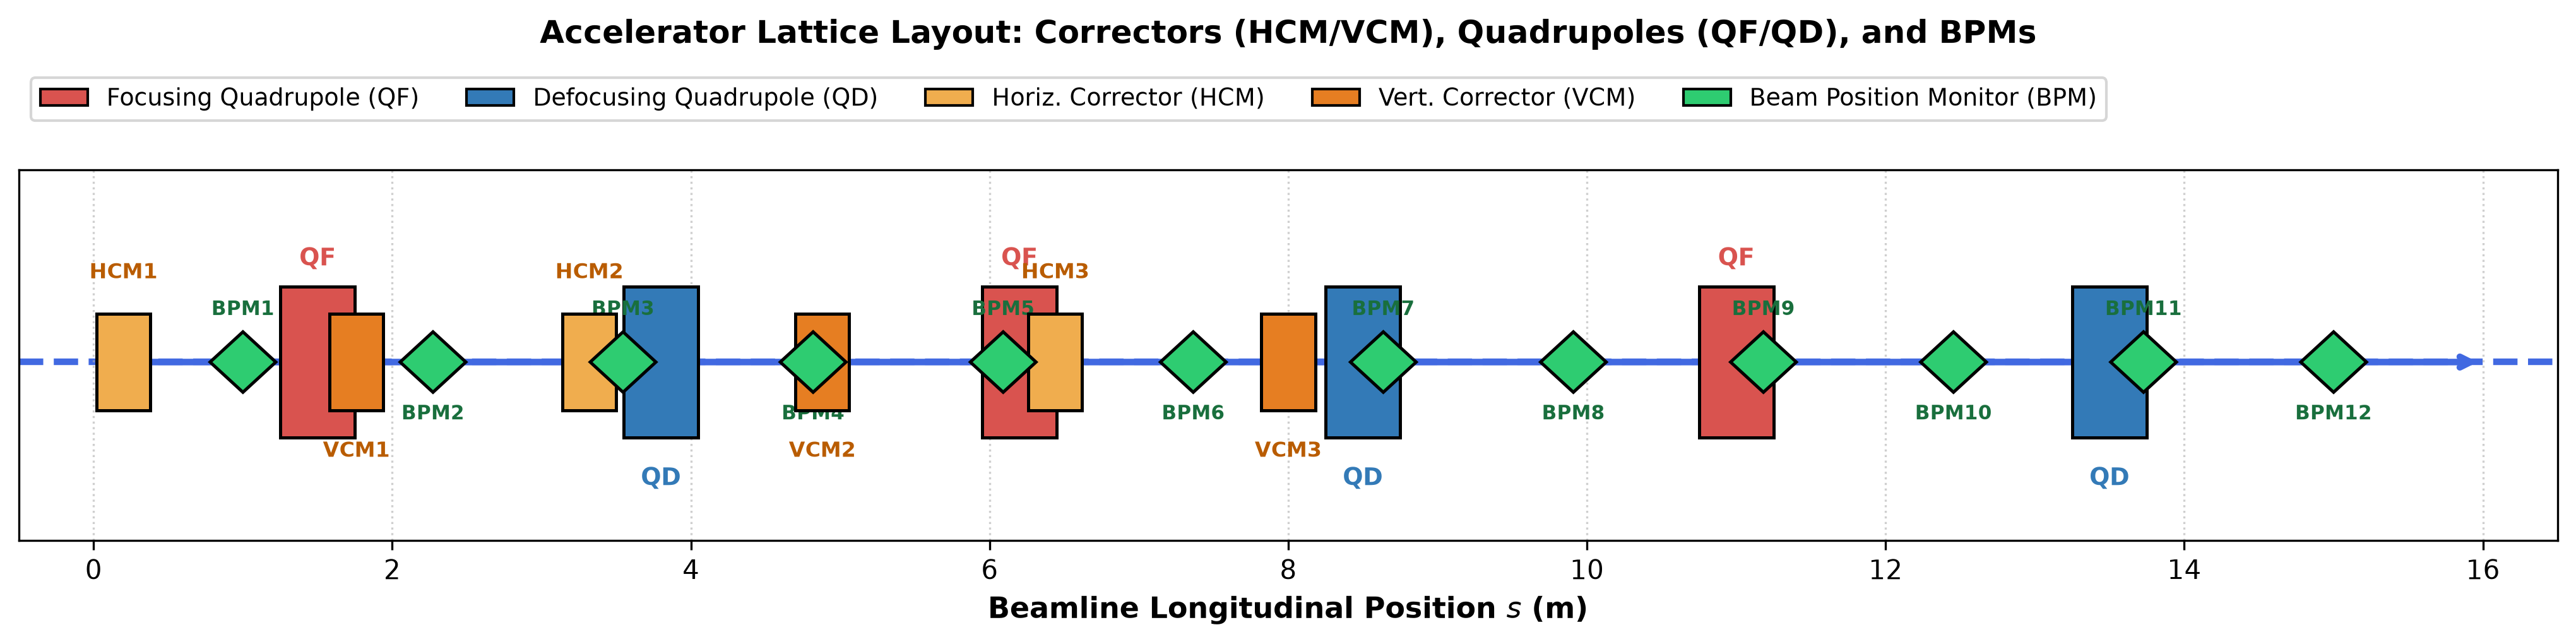
\includegraphics[width=10.0in,height=2.5in]{beamline.png}};

  % Card below at Top = 4.25in (Zero Overlap!)
  \drawcard{0.8}{4.25}{11.733}{2.45}{Transport Line Specifications \& Component Placement}
  \at{1.1}{4.8}{11.1}{\fs{13}{18}\color{darkgray}%
    $\bullet$ \textbf{12 Beam Position Monitors (BPMs):} Evenly distributed from $s = 1.0\text{ m}$ to $s = 15.0\text{ m}$, measuring transverse displacement $\mathbf{Y}$ in millimeters.\\[0.35em]
    $\bullet$ \textbf{6 Dipole Steering Magnets:} 3 Horizontal (HCM1-3) and 3 Vertical (VCM1-3) steerers positioned between $s = 0.2\text{ m}$ and $s = 8.0\text{ m}$.\\[0.35em]
    $\bullet$ \textbf{Alternating Quadrupole Doublets:} Pairs of QF and QD focusing magnets shaping the betatron phase advance and maintaining envelope stability.
  }

  \slidefooter{9}
\end{tikzpicture}
\clearpage

% ==============================================================================
% SLIDE 10: Hardware Limits & Actuator Bounds
% ==============================================================================
\begin{tikzpicture}[remember picture,overlay]
  \slidespread{1.54}
  \slideheader{Physical Limits}{Hardware Limits \& Actuator Bounds}{Realistic power supply operational boundaries and sensor measurement jitter}

  \drawcard{0.8}{1.4}{11.733}{5.3}{Power Supply Limits and Diagnostic Noise Specifications}
  \at{1.1}{2.1}{11.1}{\fs{13.5}{19}\color{darkgray}%
    {\fs{15}{18}\bfseries\color{navy}1. Cumulative Corrector Current Bounds (Thermal \& Magnetic Saturation Limit):}\\[0.3em]
    $\bullet$ Total current state: $I_k \in [-5.0\text{ A}, +5.0\text{ A}]$ for all 6 correctors.\\
    $\bullet$ Magnets entering currents $|I| > 3.0\text{ A}$ experience pronounced iron core saturation.\\
    $\bullet$ Hardware protection interlocks trip power supplies if current demands exceed $\pm 5.0\text{ A}$.\\[0.9em]
    {\fs{15}{18}\bfseries\color{navy}2. Per-Step Delta Current Bounds (Inductive Slew Rate Limit):}\\[0.3em]
    $\bullet$ Single-step control action: $\Delta I_k \in [-0.8\text{ A}, +0.8\text{ A}]$.\\
    $\bullet$ Prevents high inductive back-EMF spikes ($L \cdot \frac{di}{dt}$) that stress magnet coils and trigger power supply voltage limits.\\[0.9em]
    {\fs{15}{18}\bfseries\color{navy}3. Gaussian Diagnostic Measurement Noise (Sensor Resolution Floor):}\\[0.3em]
    $\bullet$ Sensor noise: $\epsilon_i \sim \mathcal{N}(0, \sigma^2)$, with $\sigma = 0.010\text{ mm}$ ($10\ \mu\text{m}$ RMS resolution).\\
    $\bullet$ \textbf{Crucial for control design:} Naive controllers misinterpret sensor jitter as physical orbit errors, commanding false kicks.
  }

  \slidefooter{10}
\end{tikzpicture}
\clearpage

% ==============================================================================
% SLIDE 11: Magnetic Core Non-Linear Saturation
% ==============================================================================
\begin{tikzpicture}[remember picture,overlay]
  \slidespread{1.42}
  \slideheader{Non-Linear Physics}{Magnetic Core Non-Linear Saturation}{Departing from idealized linear optics: modeling cubic saturation and quadrupole errors}

  \drawcard{0.8}{1.4}{11.733}{5.3}{Mathematical Formulation of Non-Linear Beamline Response}
  \at{1.1}{2.1}{11.1}{\fs{13.5}{19}\color{darkgray}%
    {\bfseries\color{navy}Complete Beam Position Response Formulation:}\\[0.3em]
    The actual BPM observation vector $\mathbf{Y}$ in the simulation environment is governed by:\\[0.5em]
    \centering{\fs{18}{22}\bfseries\color{primaryblue}$\mathbf{Y} = \mathbf{I} \cdot \mathbf{R}  -  0.015 \cdot ( \mathbf{I}^3 \cdot \mathbf{R} )  +  \mathbf{Y}_0  +  \boldsymbol{\epsilon}$}\\[0.7em]
    \raggedright
    {\bfseries\color{navy}$\bullet$ Physical Breakdown of Response Terms:}\\[0.3em]
    -- $\mathbf{I} \cdot \mathbf{R}$: Ideal linear betatron wave response predicted by transfer matrix.\\
    -- $-0.015 \cdot (\mathbf{I}^3 \cdot \mathbf{R})$: Non-linear iron core soft saturation. At high excitation currents, the iron yoke reaches magnetic saturation, decreasing steerer kick efficiency by 6\% (at 2 A) up to 24\% (at 4 A).\\
    -- $\mathbf{Y}_0 = \mathbf{a} \cdot \mathbf{R}$: Initial distortion from unknown kicks $a_k \sim \mathcal{U}(-2.5, 2.5)$ A at all six correctors, drawn per episode ($0.93$--$3.59\text{ mm}$ RMS on the evaluation seeds; cancelling it needs up to 2.8 A).\\
    -- $\boldsymbol{\epsilon}$: Diagnostic Gaussian measurement jitter ($\sigma = 10\ \mu\text{m}$).\\[0.8em]
    {\bfseries\color{navy}$\bullet$ Convergence Target:} \textbf{\color{successgreen}Drive orbit error below $\text{RMS} < 0.030\text{ mm}$ ($30\ \mu\text{m}$) within 50 control steps.}
  }

  \slidefooter{11}
\end{tikzpicture}
\clearpage

% ==============================================================================
% SLIDE 12: Artificial Neurons & Layer Composition
% ==============================================================================
\begin{tikzpicture}[remember picture,overlay]
  \slidespread{1.71}
  \slideheader{ML Foundations}{Artificial Neurons \& Layer Composition}{Mathematical anatomy of feedforward perceptrons and deep neural layer stacking}

  \drawcard{0.8}{1.4}{11.733}{5.3}{Neuron Transformation and Multi-Layer Composition}
  \at{1.1}{2.1}{11.1}{\fs{13.5}{19}\color{darkgray}%
    {\fs{15}{18}\bfseries\color{navy}1. The Artificial Neuron Transformation:}\\[0.3em]
    Takes input vector $\mathbf{x} \in \mathbb{R}^d$, computes affine combination, and applies non-linear activation $\sigma$:\\[0.4em]
    \centering{\fs{16}{20}\bfseries\color{primaryblue}$z = \sum_{j} w_j x_j + b = \mathbf{w}^T \mathbf{x} + b, \qquad a = \sigma(z)$}\\[0.7em]
    \raggedright
    {\fs{15}{18}\bfseries\color{navy}2. Multi-Layer Perceptron (MLP) Deep Architecture:}\\[0.3em]
    Stacks $L$ successive layers of affine transformations and non-linear activations:\\[0.4em]
    \centering{\fs{15}{18}\bfseries\color{primaryblue}$\mathbf{h}^{(l)} = \sigma\left( \mathbf{W}^{(l)} \mathbf{h}^{(l-1)} + \mathbf{b}^{(l)} \right), \quad \text{with } \mathbf{h}^{(0)} = \mathbf{x}, \quad \hat{\mathbf{y}} = \mathbf{h}^{(L)}$}\\[0.7em]
    \raggedright
    {\fs{15}{18}\bfseries\color{navy}3. Universal Approximation Theorem (Hornik et al., 1989):}\\[0.3em]
    $\bullet$ A feedforward network with at least one non-linear hidden layer can approximate any continuous non-linear function arbitrarily well, so a surrogate can represent magnetic saturation; the theorem does not say how hard such a network is to train.
  }

  \slidefooter{12}
\end{tikzpicture}
\clearpage

% ==============================================================================
% SLIDE 13: Activation Functions in Neural Networks (DEDICATED SLIDE)
% ==============================================================================
\begin{tikzpicture}[remember picture,overlay]
  \slidespread{1.14}
  \slideheader{ML Foundations}{Activation Functions in Neural Networks}{Definitions, core operational roles, non-linear mappings, and selection criteria}

  \drawcard{0.8}{1.4}{11.733}{5.3}{Activation Function Definition, Roles \& Core Comparison \hfill {\fs{11}{13}\mdseries\color{mutedgray}plots: $f(z)$ solid, $f'(z)$ dashed}}
  % Small plots of each activation f(z) (solid) and its gradient f'(z) (dashed), numbered as in the list
  \node[anchor=north east,inner sep=0pt]
    at ([xshift=12.30in,yshift=-1.95in]current page.north west)
    {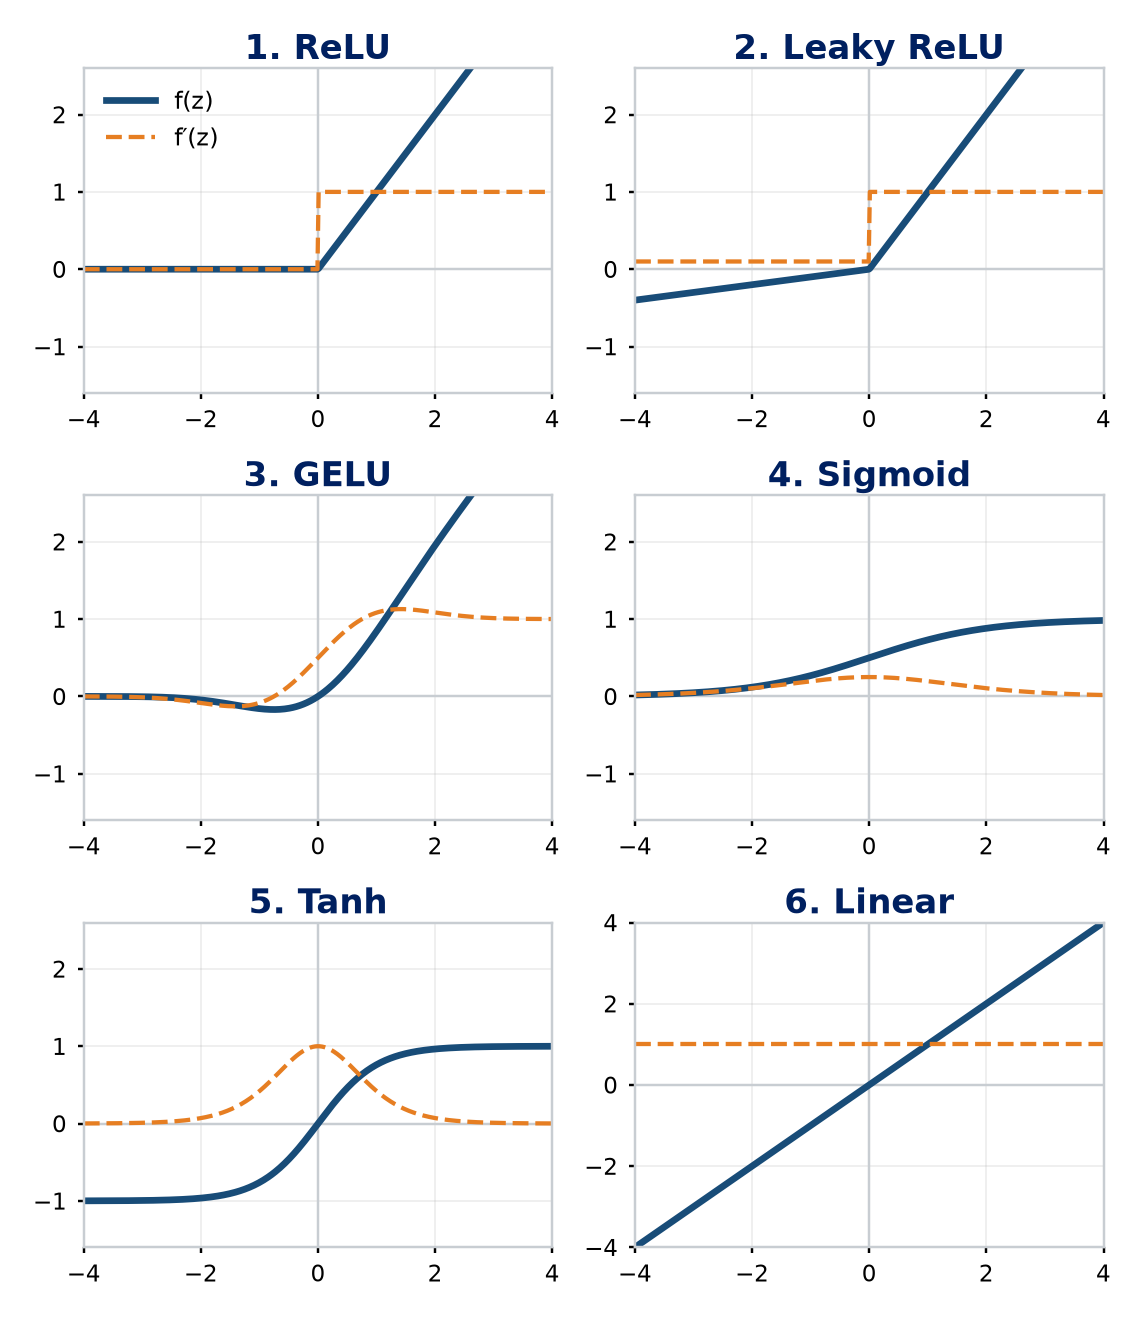
\includegraphics[height=4.50in]{activation_functions.png}};
  \at{1.1}{1.95}{7.2}{\fs{11.5}{14.5}\color{darkgray}%
    {\bfseries\color{navy}Definition \& The Four Essential Operational Roles:}\\[0.22em]
    $\bullet$ \textbf{Definition:} Non-linear mapping $\sigma(z)$ applied element-wise to pre-activation sum $z = \mathbf{w}^T \mathbf{x} + b$.\\
    $\bullet$ \textbf{Role 1 (Break Linearity):} Prevents deep layers collapsing to single matrix multiplication $\mathbf{W}_{\text{eff}}$.\\
    $\bullet$ \textbf{Role 2 (Non-Linear Physics):} Enables MLPs to approximate saturation $B(I) \propto I - 0.015 I^3$.\\
    $\bullet$ \textbf{Role 3 (Gradient Gating):} Derivative $\sigma'(z)$ regulates error flow; avoids gradient vanishing.\\
    $\bullet$ \textbf{Role 4 (Physical Bounds):} Linear activation strictly required on outputs for spatial orbits ($mm$).\\[0.45em]
    {\bfseries\color{navy}Activation Functions Catalog:}\\[0.22em]
    $\bullet$ \textbf{\color{primaryblue}1. ReLU: $f(z) = \max(0, z)$}\\
    \hspace*{1.2em}Gradient $= 1$ for $z > 0$; fast, no vanishing gradient. Default for surrogate hidden layers.\\[0.25em]
    $\bullet$ \textbf{\color{primaryblue}2. Leaky ReLU: $f(z) = \max(\alpha z, z),\ \alpha \approx 0.01$}\\
    \hspace*{1.2em}Small slope for $z < 0$ prevents ``dying'' neurons that stop learning.\\[0.25em]
    $\bullet$ \textbf{\color{primaryblue}3. GELU: $f(z) = z \cdot \Phi(z)$}\\
    \hspace*{1.2em}Smooth gating by normal CDF; standard in modern Transformers.\\[0.25em]
    $\bullet$ \textbf{\color{primaryblue}4. Sigmoid: $\sigma(z) = 1/(1 + e^{-z})$}\\
    \hspace*{1.2em}Bounded in $(0, 1)$ for probabilities; vanishes severely for $|z| > 4$.\\[0.25em]
    $\bullet$ \textbf{\color{primaryblue}5. Tanh: $\tanh(z) = (e^z - e^{-z})/(e^z + e^{-z})$}\\
    \hspace*{1.2em}Zero-centered in $(-1, 1)$; stronger gradients than Sigmoid, smooth core but saturates.\\[0.25em]
    $\bullet$ \textbf{\color{primaryblue}6. Linear / Identity: $f(z) = z$}\\
    \hspace*{1.2em}Preserves unbounded physical units; strictly mandatory for output regression layer ($\mathbf{Y}$ in mm).
  }

  \slidefooter{13}
\end{tikzpicture}
\clearpage

% ==============================================================================
% SLIDE 14: NN Surrogate Example | Learning the Particle Transfer Matrix (NEW)
% ==============================================================================
\begin{tikzpicture}[remember picture,overlay]
  \slidespread{1.22}
  \slideheader{ML Foundations}{NN Surrogate Example: Particle Transfer Matrix}{Surrogating beam optics: mapping initial phase space $(x_0, x'_0)$ to final coordinates $(x_f, x'_f)$}

  \drawcard{0.8}{1.4}{11.733}{5.3}{Surrogate Modeling of Particle Transport Matrix $\mathbf{M}$}

  % Left Column: Physics & Surrogate Equations (width 5.25 in, strictly confined to x <= 6.30 in)
  \at{1.05}{1.95}{5.25}{\fs{12}{16}\color{darkgray}%
    {\fs{13}{16}\bfseries\color{navy}1. Classical Analytical Transfer Matrix:}\\[0.25em]
    In linear beam optics, transverse particle trajectory through a beamline element is governed by the $2 \times 2$ transfer matrix $\mathbf{M}$:\\[0.3em]
    \centering{\fs{12}{15}\bfseries\color{primaryblue}$\begin{pmatrix} x_f \\ x'_f \end{pmatrix} = \mathbf{M} \begin{pmatrix} x_0 \\ x'_0 \end{pmatrix} = \begin{pmatrix} C(s) & S(s) \\ C'(s) & S'(s) \end{pmatrix} \begin{pmatrix} x_0 \\ x'_0 \end{pmatrix}, \quad \det\mathbf{M} = 1$}\\[0.3em]
    \raggedright
    $\det\mathbf{M} = 1$ ensures phase-space area preservation (Liouville's theorem / symplecticity).\\[0.8em]
    {\fs{13}{16}\bfseries\color{navy}2. Neural Network Surrogate Formulation:}\\[0.25em]
    Instead of analytical tracking, we train a neural network $f_{\boldsymbol{\theta}}: \mathbb{R}^2 \to \mathbb{R}^2$:\\[0.3em]
    \centering{\fs{11.5}{15}\bfseries\color{primaryblue}$\hat{\mathbf{z}}_f = f_{\boldsymbol{\theta}}(\mathbf{z}_0) = \mathbf{W}^{(3)}\,\sigma\Big(\mathbf{W}^{(2)}\,\sigma\big(\mathbf{W}^{(1)}\mathbf{z}_0 + \mathbf{b}^{(1)}\big) + \mathbf{b}^{(2)}\Big) + \mathbf{b}^{(3)}$}\\[0.2em]
    \centering{\fs{11}{14}\color{mutedgray}where $\mathbf{z}_0 = (x_0, x'_0)^T$ and $\hat{\mathbf{z}}_f = (\hat{x}_f, \hat{x}'_f)^T$}\\[0.7em]
    \raggedright
    {\fs{13}{16}\bfseries\color{navy}3. Supervised Objective \& Conservation Target:}\\[0.25em]
    $\bullet$ \textbf{MSE Loss:} $\mathcal{L}_{\text{MSE}} = \frac{1}{N}\sum_{i=1}^N \| \mathbf{z}_{f,i} - \hat{\mathbf{z}}_{f,i} \|_2^2$\\[0.2em]
    $\bullet$ \textbf{Jacobian Determinant (Area Conservation):}\\
    \centering{\fs{11.5}{15}\color{primaryblue}$\det \mathbf{J}_{f_{\boldsymbol{\theta}}} = \frac{\partial \hat{x}_f}{\partial x_0}\frac{\partial \hat{x}'_f}{\partial x'_0} - \frac{\partial \hat{x}_f}{\partial x'_0}\frac{\partial \hat{x}'_f}{\partial x_0} \equiv 1$}
  }

  % Right Column: TikZ Network Architecture Diagram (ENLARGED to 5.4 in x 4.4 in, starts at x = 6.75 in)
  \node[anchor=north west,inner sep=0pt] at ([xshift=6.75in,yshift=-1.95in]current page.north west) {%
    \begin{tikzpicture}[x=1in,y=1in]
      % Card background for diagram (width 5.4 in, height 4.4 in)
      \draw[rounded corners=8pt,fill=white,draw=bordergray,line width=1.0pt] (0,0.1) rectangle (5.4,-4.3);
      \node[anchor=north,text=navy,font=\bfseries\large] at (2.7, -0.05) {Neural Surrogate Architecture: $\mathbb{R}^2 \to \mathbb{R}^2$};

      % Nodes
      % Input Layer (2 nodes at x = 0.75 in)
      \node[circle,draw=primaryblue,fill=primaryblue!15,very thick,minimum size=1.05cm] (I1) at (0.75,-1.15) {\bfseries\large $x_0$};
      \node[circle,draw=primaryblue,fill=primaryblue!15,very thick,minimum size=1.05cm] (I2) at (0.75,-2.35) {\bfseries\large $x'_0$};
      \node[below=0.10cm of I2,font=\small\bfseries\color{primaryblue}] {Input $\mathbb{R}^2$};

      % Hidden Layer 1 (4 nodes at x = 2.05 in)
      \foreach \y [count=\i] in {-0.75,-1.45,-2.15,-2.85} {
        \node[circle,draw=accent,fill=accent!15,thick,minimum size=0.75cm] (H1\i) at (2.05,\y) {};
      }
      \node[below=0.08cm of H14,font=\scriptsize\bfseries\color{accent}] {Hidden 1 (4)};

      % Hidden Layer 2 (4 nodes at x = 3.35 in)
      \foreach \y [count=\i] in {-0.75,-1.45,-2.15,-2.85} {
        \node[circle,draw=accent,fill=accent!15,thick,minimum size=0.75cm] (H2\i) at (3.35,\y) {};
      }
      \node[below=0.08cm of H24,font=\scriptsize\bfseries\color{accent}] {Hidden 2 (4)};

      % Output Layer (2 nodes at x = 4.65 in)
      \node[circle,draw=successgreen,fill=successgreen!15,very thick,minimum size=1.05cm] (O1) at (4.65,-1.15) {\bfseries\large $\hat{x}_f$};
      \node[circle,draw=successgreen,fill=successgreen!15,very thick,minimum size=1.05cm] (O2) at (4.65,-2.35) {\bfseries\large $\hat{x}'_f$};
      \node[below=0.10cm of O2,font=\small\bfseries\color{successgreen}] {Output $\mathbb{R}^2$};

      % Connections
      \foreach \i in {1,2} {
        \foreach \j in {1,...,4} {
          \draw[->,>=latex,draw=primaryblue!50,line width=0.65pt] (I\i) -- (H1\j);
        }
      }
      \foreach \i in {1,...,4} {
        \foreach \j in {1,...,4} {
          \draw[->,>=latex,draw=accent!50,line width=0.65pt] (H1\i) -- (H2\j);
        }
      }
      \foreach \i in {1,...,4} {
        \foreach \j in {1,2} {
          \draw[->,>=latex,draw=successgreen!60,line width=0.65pt] (H2\i) -- (O\j);
        }
      }

      % Labels (clean vertical margin below layer titles)
      \node[anchor=north,font=\small\color{darkgray},align=center] at (2.7,-3.50) {%
        $\mathbf{W}^{(1)},\mathbf{b}^{(1)},\sigma \;\rightarrow\; \mathbf{W}^{(2)},\mathbf{b}^{(2)},\sigma \;\rightarrow\; \mathbf{W}^{(3)},\mathbf{b}^{(3)}$\\[0.25em]
        {\color{crimson}\bfseries Output activation must be Linear / Identity!}
      };
    \end{tikzpicture}
  };

  \slidefooter{14}
\end{tikzpicture}
\clearpage

% ==============================================================================
% SLIDE 15: NN Surrogate Example | Activation Functions in Beam Transport (NEW)
% ==============================================================================
\begin{tikzpicture}[remember picture,overlay]
  \slidespread{1.16}
  \slideheader{ML Foundations}{NN Surrogate: Activation Functions in Beam Transport}{How choice of activation function governs phase space distortion, symplecticity, and extrapolation}

  \drawcard{0.8}{1.4}{11.733}{5.3}{Behavior of Activation Functions on Phase Space $(x, x')$ and Transfer Matrix $\mathbf{M}$}

  % Left Column (Width = 5.4 in)
  \at{1.1}{1.95}{5.4}{\fs{11.5}{15}\color{darkgray}%
    {\fs{13}{16}\bfseries\color{navy}1. Linear / Identity Activation ($\sigma(z) = z$):}\\[0.25em]
    $\bullet$ \textbf{Matrix Collapse:} Stacking linear layers mathematically collapses to $\mathbf{W}^{(L)} \cdots \mathbf{W}^{(1)}\mathbf{x} + \mathbf{b} \equiv \mathbf{M}_{\text{eff}}\mathbf{x} + \mathbf{b}$. The network is identical to a transfer matrix.\\
    $\bullet$ \textbf{Beam Optics Impact:} Exactly preserves linear phase-space ellipses ($\gamma x^2 + 2\alpha x x' + \beta x'^2 = \epsilon$) and symplecticity ($\det\mathbf{M}_{\text{eff}} = 1$). Extrapolates perfectly to large beam sizes.\\
    $\bullet$ \textbf{Limitation:} Fundamentally incapable of learning non-linear chromaticity, sextupole kicks ($x' \propto x^2$), or magnetic core saturation.\\[1.0em]
    {\fs{13}{16}\bfseries\color{navy}2. Rectified Linear Unit (ReLU: $\max(0, z)$):}\\[0.25em]
    $\bullet$ \textbf{Piecewise Linear Facets:} Partitions phase space $(x, x')$ into polyhedral regions bounded by hyperplanes $\mathbf{w}_j^T \mathbf{x} + b_j = 0$. Within each region, mapping is affine.\\
    $\bullet$ \textbf{Beam Optics Impact:} Deforms smooth phase-space ellipses into \textbf{faceted polygons with sharp slope kinks} (non-differentiable corners).\\
    $\bullet$ \textbf{Dying Neurons Risk:} Particles entering inactive half-spaces ($z < 0$) have zero gradient and output 0, collapsing phase space volume ($\det \mathbf{J} = 0$) and violating Liouville's theorem.
  }

  % Right Column (Width = 5.4 in)
  \at{6.85}{1.95}{5.4}{\fs{11.5}{15}\color{darkgray}%
    {\fs{13}{16}\bfseries\color{navy}3. Hyperbolic Tangent (Tanh: $\tanh(z)$):}\\[0.25em]
    $\bullet$ \textbf{Smooth Non-Linearity:} Continuously differentiable ($C^\infty$). Near the core ($|z| \ll 1$), $\tanh(z) \approx z$, accurately recovering linear optics $\mathbf{M}$.\\
    $\bullet$ \textbf{Halo Saturation Distortion:} At large amplitudes (beam halo or large steering errors), hidden neurons \textbf{saturate} ($\tanh(z) \to \pm 1$). Squashes phase-space ellipses into S-curves, artificially compressing emittance ($\det\mathbf{J} \to 0$) and violating symplecticity in the wings.\\
    $\bullet$ \textbf{Extrapolation Danger:} Bounded non-linearities fail to extrapolate outside the training current envelope.\\[1.0em]
    {\fs{13}{16}\bfseries\color{navy}4. Output Layer Architecture Requirement:}\\[0.25em]
    $\bullet$ \textbf{\color{crimson}Strictly Linear (Identity) Output:}\\
    Transverse coordinates $x_f$ and angles $x'_f$ are unbounded real values ($mm, mrad$).\\
    $\bullet$ \textbf{Aperture Clipping Hazard:} Applying a bounded activation (Tanh / Sigmoid) on output neurons artificially clamps beam trajectories, imposing an unphysical numerical collimator!
  }

  \slidefooter{15}
\end{tikzpicture}
\clearpage

% ==============================================================================
% SLIDE 16: Optimization Algorithms in Machine Learning (DEDICATED SLIDE)
% ==============================================================================
\begin{tikzpicture}[remember picture,overlay]
  \slidespread{1.26}
  \slideheader{ML Foundations}{Optimization Algorithms in Machine Learning}{First-order stochastic gradient methods, momentum, adaptive learning rates, and quasi-Newton solvers}

  \drawcard{0.8}{1.4}{11.733}{5.3}{Evolution of Solvers: From Standard SGD to Adam and L-BFGS-B}

  % Left Column (Width = 5.4 in)
  \at{1.1}{1.95}{5.4}{\fs{11.5}{16}\color{darkgray}%
    {\fs{13}{16.5}\bfseries\color{navy}Classical First-Order \& Adaptive Solvers:}\\[0.4em]
    {\bfseries\color{navy}1. SGD (Stochastic Gradient Descent):}\\[0.15em]
    $\bullet$ \textbf{\color{primaryblue}$\boldsymbol{\theta} \leftarrow \boldsymbol{\theta} - \eta \cdot \mathbf{g}$}: Basic first-order parameter update.\\
    $\bullet$ Highly sensitive to learning rate $\eta$; oscillates violently across steep, narrow ravines in accelerator parameter space.\\[1.1em]
    {\bfseries\color{navy}2. Momentum SGD:}\\[0.15em]
    $\bullet$ \textbf{\color{primaryblue}$\mathbf{v} \leftarrow \gamma \mathbf{v} + \eta \mathbf{g}, \quad \boldsymbol{\theta} \leftarrow \boldsymbol{\theta} - \mathbf{v}$}: Accumulates velocity ($\gamma \approx 0.9$).\\
    $\bullet$ Dampens high-frequency oscillations across ravine walls; accelerates along flat valley floors toward optimal minima.\\[1.1em]
    {\bfseries\color{navy}3. AdaGrad \& RMSProp:}\\[0.15em]
    $\bullet$ \textbf{\color{primaryblue}AdaGrad}: Adapts per-parameter step sizes via $\sum \mathbf{g}^2$; however, learning rate decays monotonically to zero.\\
    $\bullet$ \textbf{\color{primaryblue}RMSProp}: Uses exponentially decaying average of squared gradients $\mathbf{v} \leftarrow \beta \mathbf{v} + (1-\beta)\mathbf{g}^2$, preventing premature freeze.
  }

  % Right Column (Width = 5.4 in)
  \at{6.85}{1.95}{5.4}{\fs{11.5}{16}\color{darkgray}%
    {\fs{13}{16.5}\bfseries\color{navy}Advanced Solvers \& Quasi-Newton Inversion:}\\[0.4em]
    {\bfseries\color{navy}4. Adam (Adaptive Moment Estimation):}\\[0.15em]
    $\bullet$ \textbf{\color{primaryblue}Combines Momentum + RMSProp + Bias Correction}:\\
    $\mathbf{m}_t = \beta_1 \mathbf{m}_{t-1} + (1-\beta_1)\mathbf{g}_t, \quad \mathbf{v}_t = \beta_2 \mathbf{v}_{t-1} + (1-\beta_2)\mathbf{g}_t^2$\\
    $\bullet$ \textbf{Surrogate Gold Standard:} Automatically scales steps across heterogeneous magnet corrector channels.\\[1.1em]
    {\bfseries\color{navy}5. AdamW (Decoupled Weight Decay):}\\[0.15em]
    $\bullet$ \textbf{\color{primaryblue}Decouples $L_2$ Regularization from Gradient Updates}:\\
    Subtracts weight decay directly ($\boldsymbol{\theta} \leftarrow \boldsymbol{\theta} - \eta \lambda \boldsymbol{\theta}$), yielding superior holdout generalization on noisy BPM data.\\[1.1em]
    {\bfseries\color{navy}6. L-BFGS-B (Quasi-Newton with Box Bounds):}\\[0.15em]
    $\bullet$ \textbf{\color{primaryblue}Second-Order Inverse Hessian Approximation}:\\
    Computes curvature from gradient history without storing full $N \times N$ matrix. Standard for bounded model inversion (Baseline 1 \& Track 3).
  }

  \slidefooter{16}
\end{tikzpicture}
\clearpage

% ==============================================================================
% SLIDE 17: Neural Architectures Beyond MLPs: PINN, PRNN, VAE & U-Net (NEW)
% ==============================================================================
\begin{tikzpicture}[remember picture,overlay]
  \slidespread{1.10}
  \slideheader{ML Foundations}{Specialized Neural Architectures: Beyond Plain MLPs}{Domain-adapted deep learning topologies tailored to accelerator physics, time dynamics, and imaging}

  \drawcard{0.8}{1.4}{11.733}{5.3}{Taxonomy of Specialized Deep Learning Architectures in Particle Accelerators}

  % 1. PINN Panel (Top-Left: x=1.00, y=1.95, w=5.40, h=2.15)
  \draw[rounded corners=4pt,draw=primaryblue!45,fill=primaryblue!4,thick]
    ([xshift=1.00in,yshift=-1.95in]current page.north west) rectangle ++(5.40in,-2.17in);
  \at{1.12}{2.05}{5.15}{\fs{10.5}{13.5}\color{darkgray}%
    {\fs{12}{14}\bfseries\color{primaryblue}1. PINN: Physics-Informed Neural Networks}\\[0.25em]
    $\bullet$ \textbf{Mechanism:} Embeds governing ODEs/PDEs directly into the training loss:
    $$\mathcal{L}_{\text{PINN}} = \mathcal{L}_{\text{data}} + \lambda_{\text{phys}}\,\big\|\mathcal{D}[f_{\boldsymbol{\theta}}](\mathbf{x})\big\|^2$$\\[-0.5em]
    where differential operator $\mathcal{D}$ is evaluated via exact automatic differentiation.\\
    $\bullet$ \textbf{Why Beyond MLP:} Enforces physical conservation (energy, symplecticity $\det\mathbf{J}\equiv 1$) even in data-sparse regimes where MLPs produce unphysical drift.\\
    $\bullet$ \textbf{Accelerator Use:} Space-charge Poisson solvers, beam envelope tracking, and trajectory prediction across unmonitored lattice drift sections.
  }

  % 2. PRNN / RNN Panel (Top-Right: x=6.75, y=1.95, w=5.40, h=2.15)
  \draw[rounded corners=4pt,draw=accent!50,fill=accent!4,thick]
    ([xshift=6.75in,yshift=-1.95in]current page.north west) rectangle ++(5.40in,-2.17in);
  \at{6.87}{2.05}{5.15}{\fs{10.5}{13.5}\color{darkgray}%
    {\fs{12}{14}\bfseries\color{accent}2. PRNN / RNN: Physics-Guided Recurrent Networks}\\[0.25em]
    $\bullet$ \textbf{Mechanism:} Sequential state transitions with internal dynamic memory:
    $$\mathbf{h}_t = \sigma(\mathbf{W}_h \mathbf{h}_{t-1} + \mathbf{W}_x \mathbf{x}_t + \mathbf{b}_h)$$\\[-0.5em]
    augmented with physics inductive biases (e.g., hysteresis models, thermal delay).\\
    $\bullet$ \textbf{Why Beyond MLP:} MLPs assume independent static inputs; PRNNs model non-Markovian memory, temporal lags, and hysteretic state dependence.\\
    $\bullet$ \textbf{Accelerator Use:} Magnet iron hysteresis tracking during cycling, superconducting RF cavity decay, and precursor thermal drift forecasting.
  }

  % 3. VAE Panel (Bottom-Left: x=1.00, y=4.28, w=5.40, h=2.15)
  \draw[rounded corners=4pt,draw=successgreen!50,fill=successgreen!4,thick]
    ([xshift=1.00in,yshift=-4.28in]current page.north west) rectangle ++(5.40in,-2.17in);
  \at{1.12}{4.38}{5.15}{\fs{10.5}{13.5}\color{darkgray}%
    {\fs{12}{14}\bfseries\color{successgreen}3. VAE: Variational Autoencoders}\\[0.25em]
    $\bullet$ \textbf{Mechanism:} Probabilistic encoder-decoder mapping inputs to latent Gaussian distribution $\mathbf{z} \sim \mathcal{N}(\boldsymbol{\mu}, \boldsymbol{\Sigma})$, optimizing the Evidence Lower Bound:
    $$\mathcal{L}_{\text{ELBO}} = \mathbb{E}_{q}[\log p_{\boldsymbol{\theta}}(\mathbf{x}|\mathbf{z})] - D_{\text{KL}}\big(q_{\boldsymbol{\phi}}(\mathbf{z}|\mathbf{x})\,\|\,p(\mathbf{z})\big)$$\\[-0.5em]
    $\bullet$ \textbf{Why Beyond MLP:} Learns continuous, structured generative latent manifolds rather than deterministic black-box point mappings.\\
    $\bullet$ \textbf{Accelerator Use:} 6D particle bunch phase-space compression, unsupervised anomaly/trip detection, and synthetic generative beam diagnostics.
  }

  % 4. U-Net / CNN Panel (Bottom-Right: x=6.75, y=4.28, w=5.40, h=2.15)
  \draw[rounded corners=4pt,draw=gold!60,fill=gold!4,thick]
    ([xshift=6.75in,yshift=-4.28in]current page.north west) rectangle ++(5.40in,-2.17in);
  \at{6.87}{4.38}{5.15}{\fs{10.5}{13.5}\color{darkgray}%
    {\fs{12}{14}\bfseries\color{gold}4. U-Net / CNN: Convolutional Encoder-Decoders}\\[0.25em]
    $\bullet$ \textbf{Mechanism:} Contracting feature extraction path paired with symmetric upsampling path, bridged by multiscale cross-layer skip connections:
    $$\mathbf{x}_{\text{dec}}^{(l)} = \text{Conv}\big(\text{Upsample}(\mathbf{x}_{\text{dec}}^{(l+1)}) \;\oplus\; \mathbf{x}_{\text{enc}}^{(l)}\big)$$\\[-0.5em]
    $\bullet$ \textbf{Why Beyond MLP:} Exploits 2D/3D spatial translation equivariance; retains high-resolution local details while capturing global topological context.\\
    $\bullet$ \textbf{Accelerator Use:} YAG/OTR beam screen image reconstruction, transverse halo segmentation, phase-space tomography, and 3D magnet field interpolation.
  }

  \slidefooter{17}
\end{tikzpicture}
\clearpage

% SLIDE 18: Paradigm 1: Supervised Learning | Digital Twin Surrogates & Hyperparameters (NEW)
% ==============================================================================
\begin{tikzpicture}[remember picture,overlay]
  \slidespread{1.18}
  \slideheader{Paradigm 1}{Supervised Learning: Digital Twins \& Hyperparameters}{Training data-driven accelerator forward surrogates to model complex non-linear optics}

  \drawcard{0.8}{1.4}{11.733}{5.3}{Supervised Learning Workflow, Optimization \& Hyperparameter Taxonomy}

  % Left column: How it works + Terminology (width 4.95 in, starts at x = 1.05 in, y = 1.95 in)
  \at{1.05}{1.95}{4.95}{\fs{11.5}{16}\color{darkgray}%
    {\bfseries\color{navy}1. Core Model Training Terminology \& Workflow:}\\[0.55em]
    $\bullet$ \textbf{Weights $\mathbf{W}$ \& Biases $\mathbf{b}$:} Trainable synaptic multipliers and threshold offsets updated during learning.\\[0.65em]
    $\bullet$ \textbf{Loss Function $\mathcal{L}(\boldsymbol{\theta})$:} Error metric (MSE) measuring discrepancy between predicted orbit $\hat{\mathbf{Y}}$ and true BPM vector $\mathbf{Y}$.\\[0.65em]
    $\bullet$ \textbf{Gradient \& Backpropagation:} Multivariable chain rule propagating loss gradients $\nabla_{\boldsymbol{\theta}}\mathcal{L}$ backward to compute weight steps.\\[0.65em]
    $\bullet$ \textbf{Epoch vs Batch vs Step / Iteration:}\\[0.28em]
    \hspace*{0.8em}-- \emph{Epoch:} One complete training pass through the full dataset ($N$ shots).\\[0.25em]
    \hspace*{0.8em}-- \emph{Batch ($B$):} Subset of training shots evaluated per gradient step.\\[0.25em]
    \hspace*{0.8em}-- \emph{Step / Iteration:} A single weight vector update $\boldsymbol{\theta} \leftarrow \boldsymbol{\theta} - \Delta\boldsymbol{\theta}$.\\[0.65em]
    $\bullet$ \textbf{Generalization \& Early Stopping:} Halts training when validation loss stops improving, avoiding memorizing sensor noise ($10\ \mu\text{m}$).
  }

  % Right column: Hyperparameters Taxonomy Table (width 5.75 in, starts at x = 6.40 in, y = 1.95 in)
  \node[anchor=north west,inner sep=0pt]
    at ([xshift=6.40in,yshift=-1.95in]current page.north west) {%
      \fs{10.5}{13.5}\color{darkgray}%
      \renewcommand{\arraystretch}{1.14}
      \setlength{\tabcolsep}{5pt}
      \begin{tabular}{@{}p{1.35in}p{1.30in}p{2.85in}@{}}
        \toprule
        \textbf{\color{primaryblue}Hyperparameter} & \textbf{\color{primaryblue}Typical Value} & \textbf{\color{primaryblue}Physical Meaning \& Effect on Model} \\
        \midrule
        \textbf{\color{tunablered}Learning Rate ($\eta$)$^*$} & $10^{-3}$ (Adam) & Step size along gradient. Too large diverges; too small stagnates in local plateaus. \\
        \textbf{\color{tunablered}Batch Size ($B$)$^*$} & 32 to 128 & Samples per gradient step. Smaller batches provide stochastic regularization; larger give speed. \\
        \textbf{\color{tunablered}Architecture$^*$} & (128, 64, 32) & Depth and width. Must have capacity to capture cubic saturation without memorizing noise. \\
        \textbf{\color{tunablered}Activation ($\sigma$)$^*$} & \texttt{relu}, \texttt{tanh} & Non-linearity in hidden layers. The output layer is always linear. \\
        \textbf{\color{tunablered}Solver$^*$} & \texttt{adam}, \texttt{lbfgs} & Training algorithm. \texttt{lbfgs} is full-batch and suits small, smooth datasets. \\
        \textbf{\color{tunablered}L2 Penalty ($\alpha$)$^*$} & $10^{-4}$ & Weight decay penalty $\frac{1}{2}\alpha\|\mathbf{w}\|^2$. Suppresses overfitting to BPM jitter ($10\ \mu\text{m}$). \\
        \textbf{\color{tunablered}Max Epochs / Tol$^*$} & 400 epochs, tol=$10^{-4}$ & Stops when the loss improves by less than tol (about 85 epochs by default). \\
        \bottomrule
        \multicolumn{3}{@{}l@{}}{\fs{9}{12}\color{tunablered}\bfseries * Red text: Hyperparameters participants can modify in notebook TODO 1}\\[-0.2em]
      \end{tabular}
    };

  \slidefooter{18}
\end{tikzpicture}
\clearpage

% ==============================================================================
% SLIDE 19: Neural Surrogate Digital Twin (RESIZED - ZERO OVERLAP)
% ==============================================================================
\begin{tikzpicture}[remember picture,overlay]
  \slidespread{1.15}
  \slideheader{Surrogate Modeling}{Neural Surrogate Digital Twin}{Deep Multi-Layer Perceptron (128-64-32) capturing non-linear cubic saturation}

  % Sized Image: Height = 3.85 in (aspect ratio preserved)
  \node[anchor=north,inner sep=0pt]
    at ([yshift=-1.40in]current page.north)
    {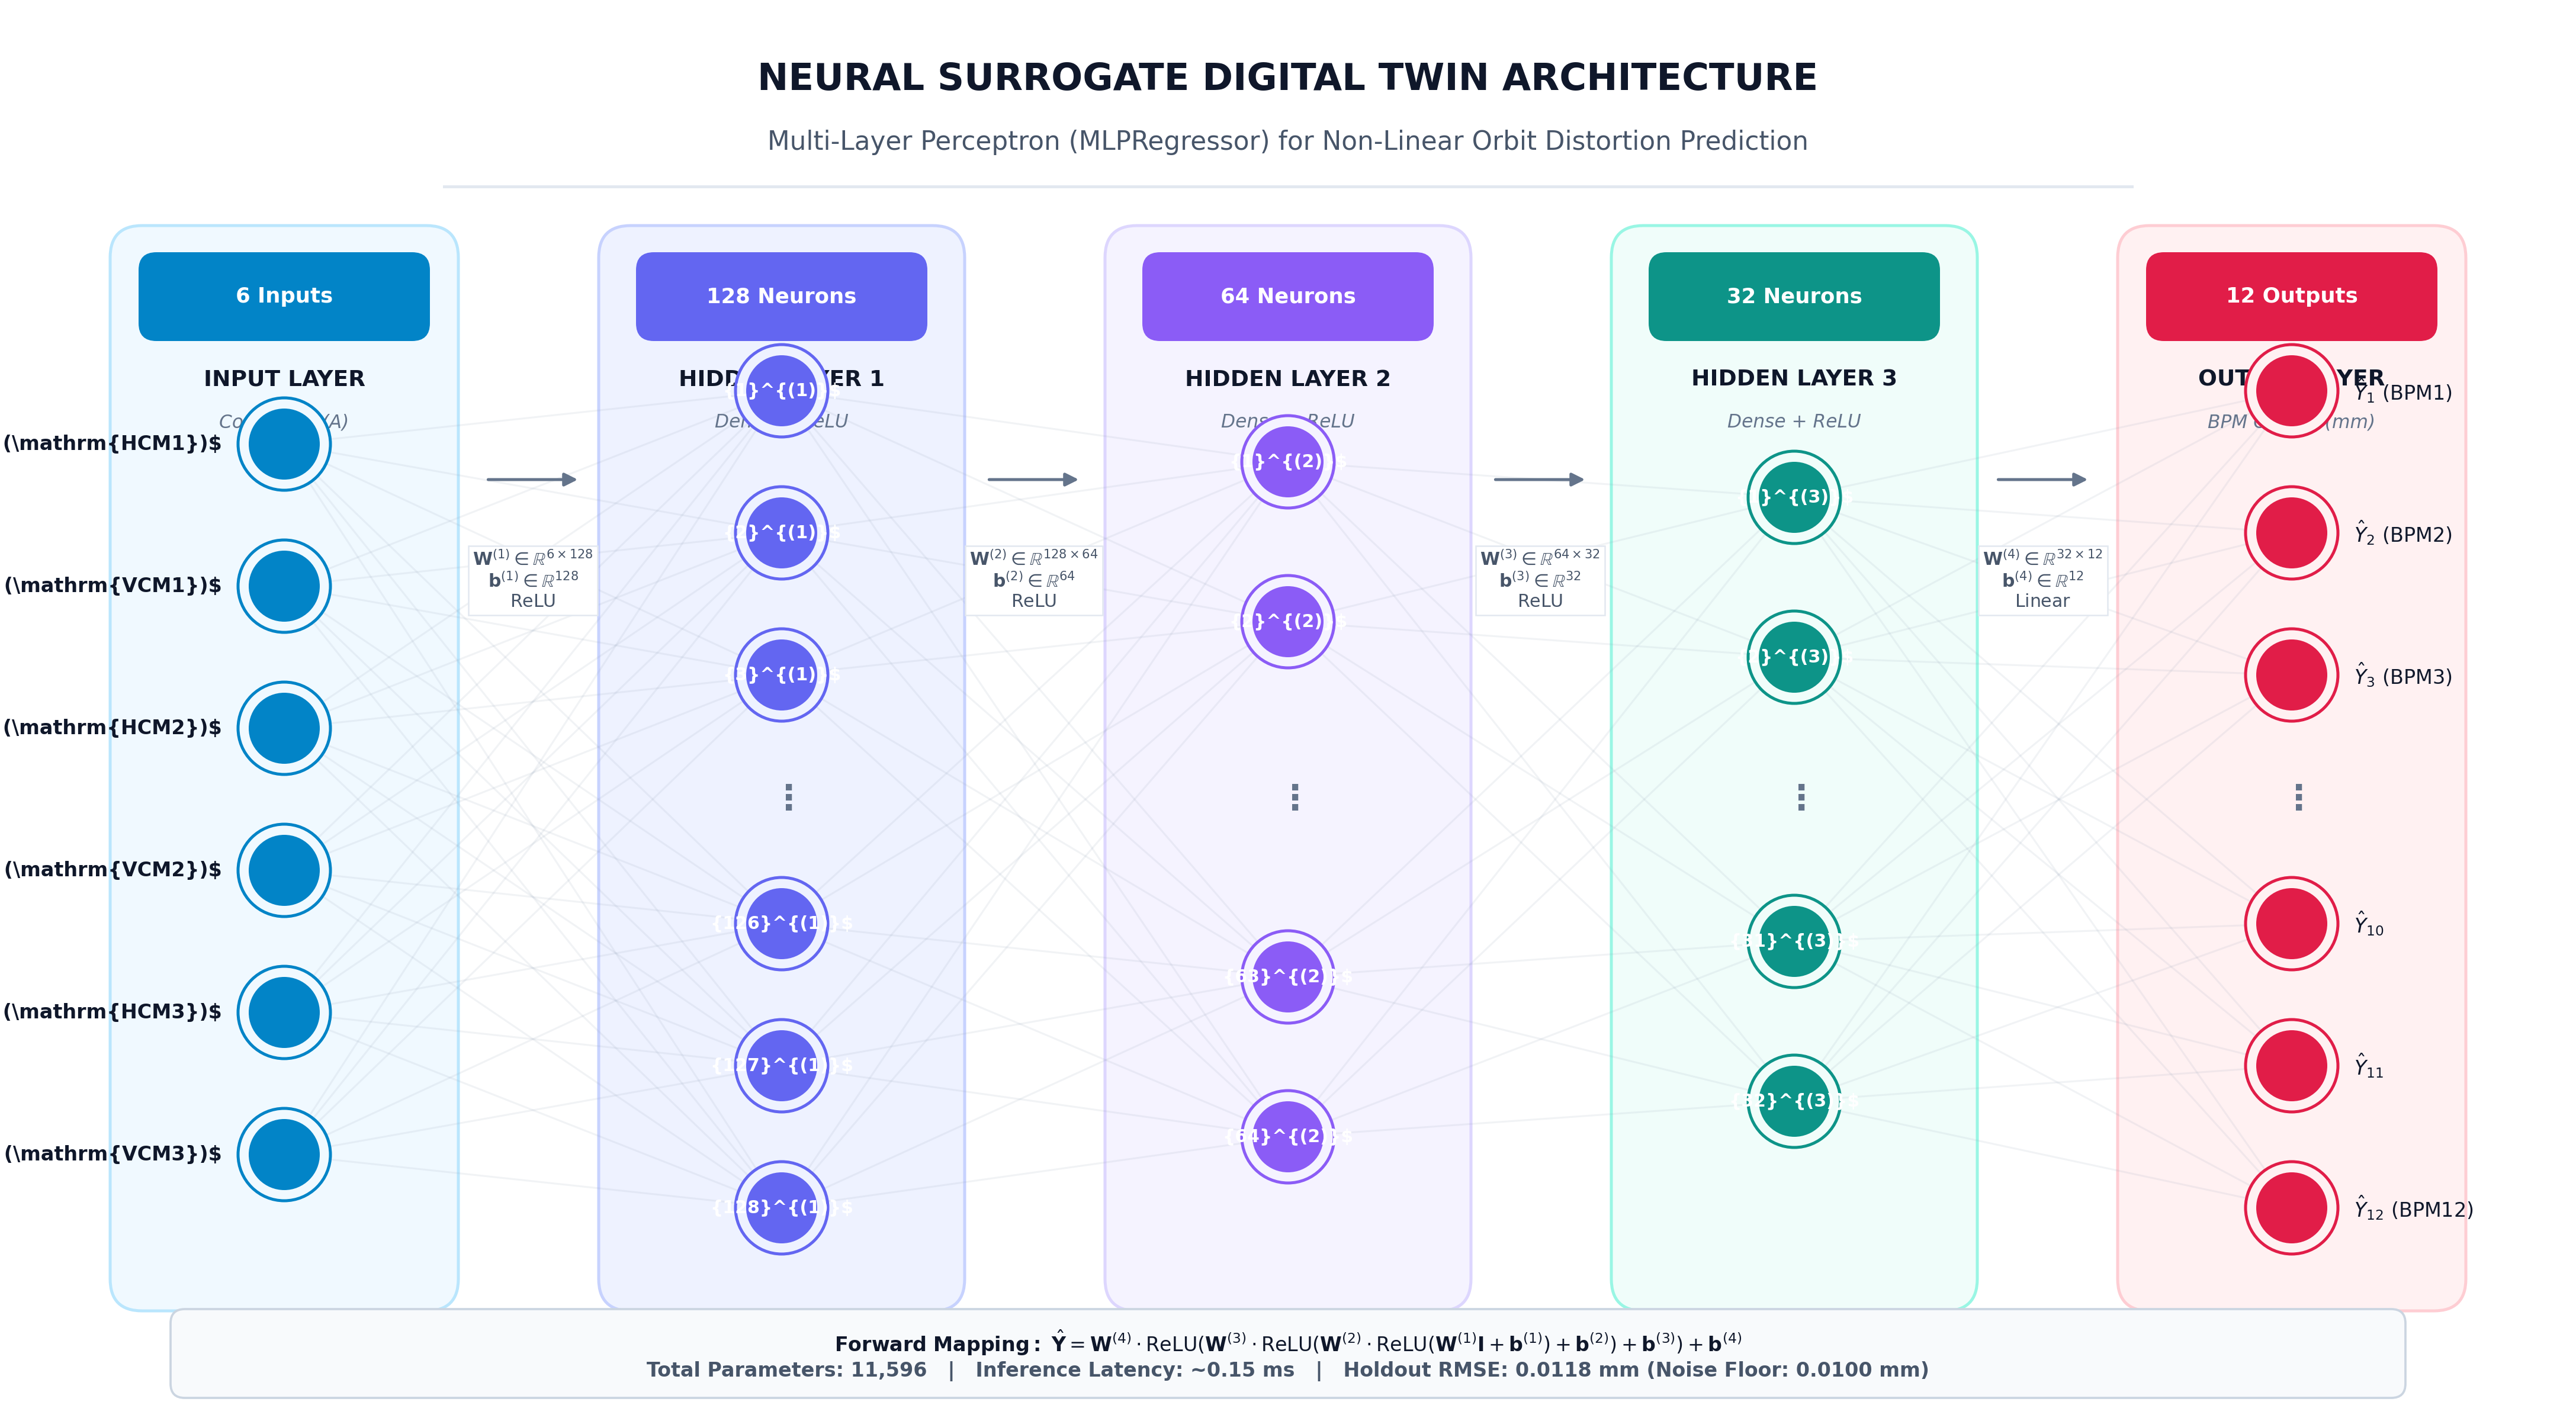
\includegraphics[height=3.85in]{mlp_schematic.png}};

  % Card below the image
  \drawcard{0.8}{5.38}{11.733}{1.22}{}
  \node[anchor=west,inner sep=0pt,text width=11.3in,align=left]
    at ([xshift=1.0in,yshift=-5.99in]current page.north west) {\fs{12}{15}\color{darkgray}%
    $\bullet$ \textbf{Input Layer:} 6 Corrector Magnet Currents [HCM1-3, VCM1-3] in Amperes.\\[0.1em]
    $\bullet$ \textbf{Hidden Layers:} Dense layers ($128 \rightarrow 64 \rightarrow 32$) with ReLU non-linear activations capturing cubic iron-core saturation.\\[0.1em]
    $\bullet$ \textbf{Output Layer:} 12 predicted Beam Position Monitor readings [BPM1-12] in millimeters, evaluated in $< 0.2\text{ milliseconds}$.
  };

  \slidefooter{19}
\end{tikzpicture}
\clearpage

% ==============================================================================
% SLIDE 20: Surrogate Training & Holdout Validation
% ==============================================================================
\begin{tikzpicture}[remember picture,overlay]
  \slidespread{1.27}
  \slideheader{Digital Twin Validation}{Surrogate Training \& Validation}{Ensuring digital twin fidelity across linear and saturated magnetic operating regimes}

  \drawcard{0.8}{1.4}{11.733}{5.3}{Offline Dataset Generation and Model Verification}
  \at{1.1}{2.1}{11.1}{\fs{13.5}{19}\color{darkgray}%
    {\fs{15}{18}\bfseries\color{navy}1. Offline Dataset (notebook Step 3):}\\[0.3em]
    $\bullet$ 1,500 simulated shots with corrector currents sampled uniformly in $\mathbf{I} \in [-3.0, +3.0]^6\text{ A}$ (the correction needs up to 2.84 A).\\
    $\bullet$ Full non-linear response including the cubic term $-0.015 \cdot (\mathbf{I}^3 \cdot \mathbf{R})$ and $10\ \mu\text{m}$ sensor noise.\\
    $\bullet$ Split into 80\% training (1,200 shots) and 20\% holdout test (300 shots), never used for training.\\[0.9em]
    {\fs{15}{18}\bfseries\color{navy}2. Holdout Test RMSE (sensor noise floor: 0.010 mm):}\\[0.3em]
    $\bullet$ \textbf{Linear Ridge} (84 parameters): $0.082\text{ mm}$. Misses the saturation.\\
    $\bullet$ \textbf{Reference MLP} (ReLU, Adam, 128-64-32; 11,628 parameters): $0.109\text{ mm}$. Adam stops after about 85 epochs, and the network predicts \textbf{worse than the linear model}.\\
    $\bullet$ \textbf{Tuned MLP} (\texttt{tanh}, \texttt{lbfgs}, 64-64; 5,388 parameters): \textbf{\color{successgreen}$0.012\text{ mm}$}, close to the noise floor.\\[0.9em]
    {\fs{15}{18}\bfseries\color{navy}3. Lessons:}\\[0.3em]
    $\bullet$ A larger network is not automatically a better surrogate: always check the holdout RMSE (\textbf{TODO 1}).\\
    $\bullet$ No model can beat the $0.010\text{ mm}$ noise floor on noisy test data. Inference takes about $0.1\text{ ms}$ per call.
  }
  \slidefooter{20}
\end{tikzpicture}
\clearpage

% ==============================================================================
% SLIDE 21: Closed-Loop Control Architecture (RESIZED - ZERO OVERLAP)
% ==============================================================================
\begin{tikzpicture}[remember picture,overlay]
  \slidespread{1.15}
  \slideheader{Closed-Loop Control}{Closed-Loop Control Architecture}{Three learning paradigms behind the challenge tracks; all three act on the measured orbit at every step}

  % Sized Image: Height = 3.85 in (aspect ratio preserved)
  \node[anchor=north,inner sep=0pt]
    at ([yshift=-1.40in]current page.north)
    {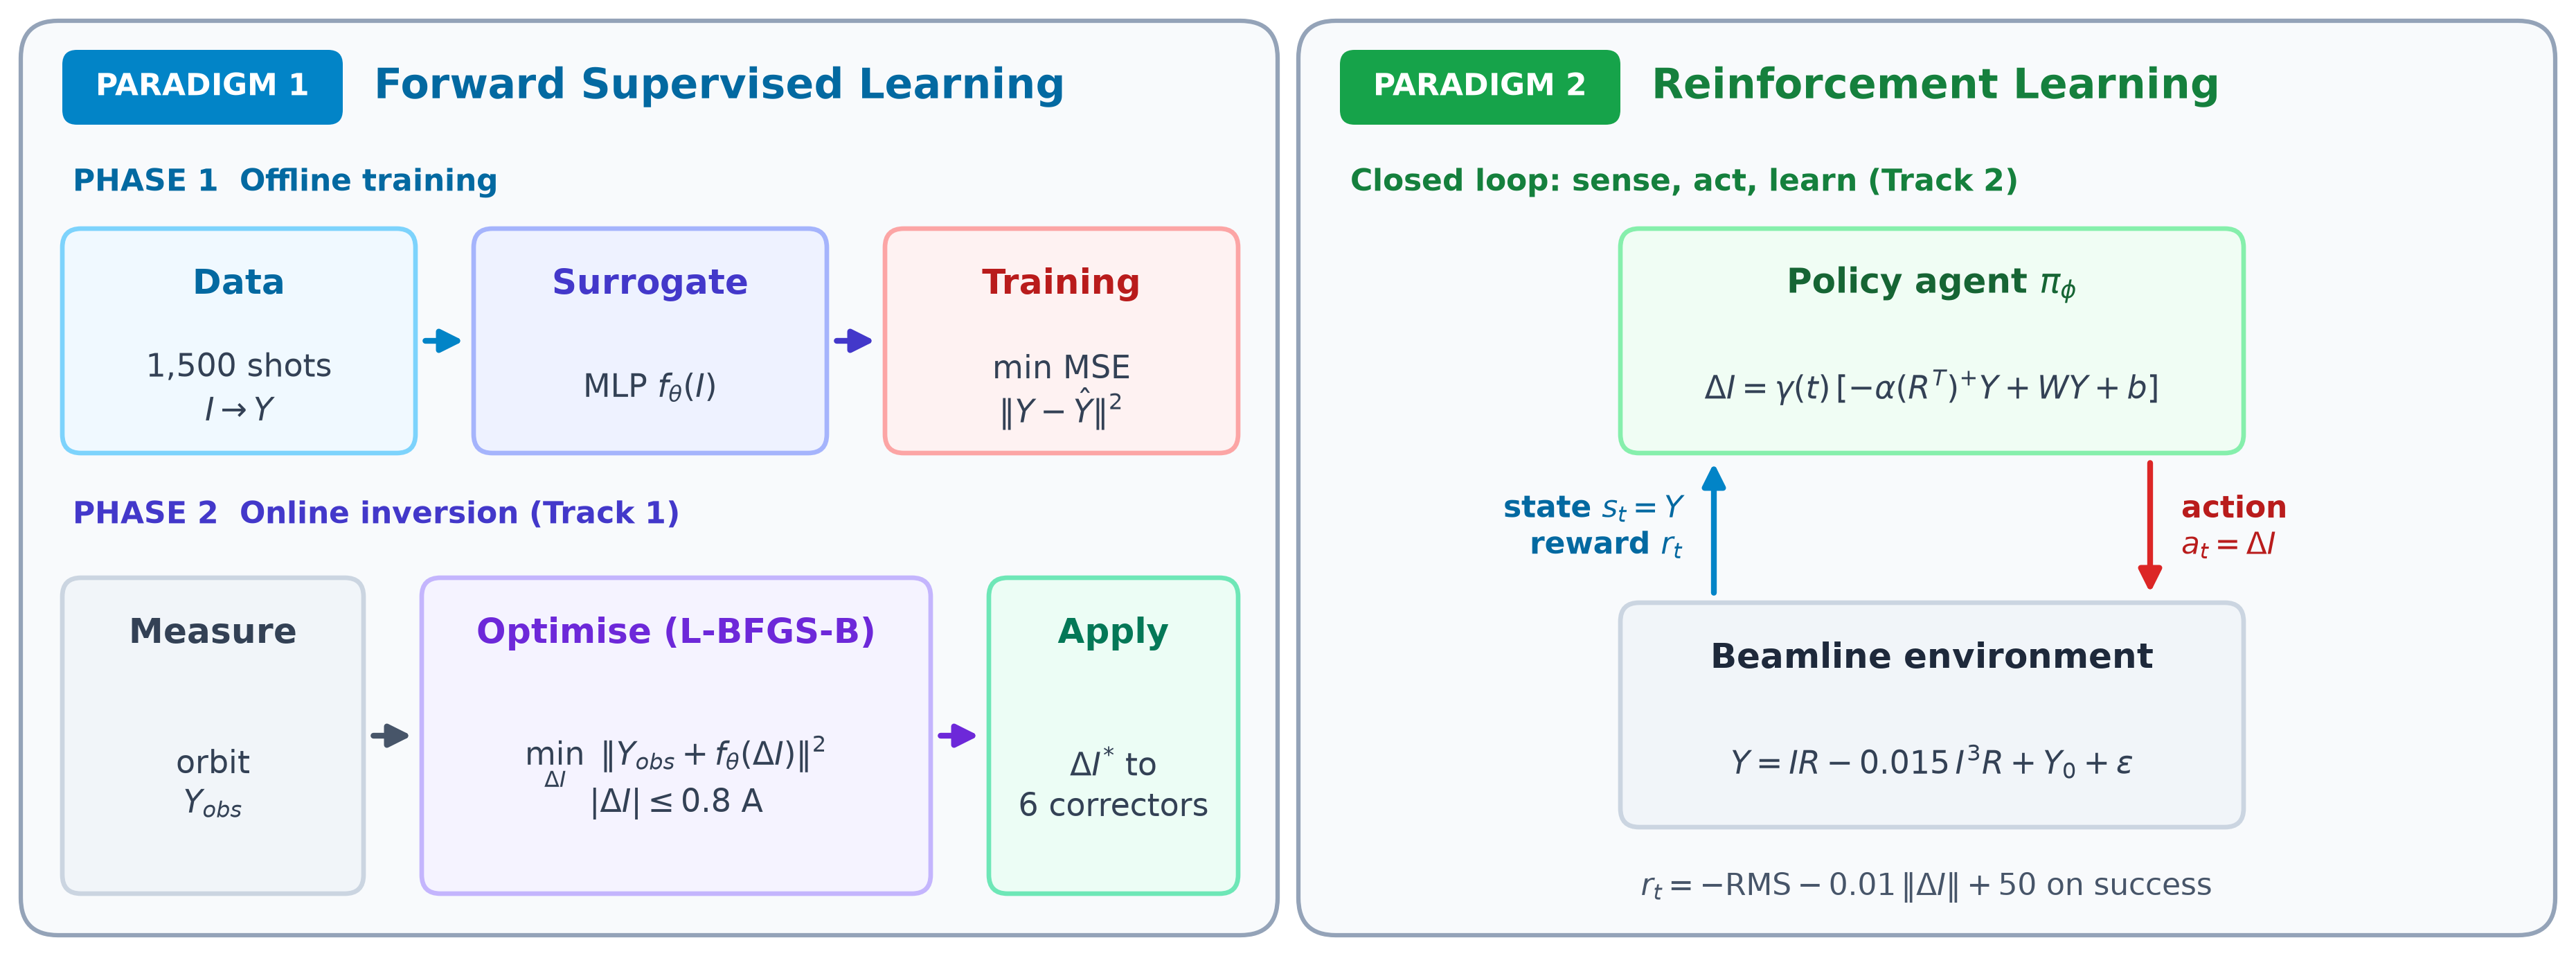
\includegraphics[height=3.85in]{forward_sl_and_rl_schematic.png}};

  % Card below the image
  \drawcard{0.8}{5.38}{11.733}{1.22}{}
  \node[anchor=west,inner sep=0pt,text width=11.3in,align=left]
    at ([xshift=1.0in,yshift=-5.99in]current page.north west) {\fs{12}{15}\color{darkgray}%
    $\bullet$ \textbf{Supervised (Track 1):} trains an MLP surrogate offline, then inverts it at each step for the kick $\Delta\mathbf{I}$.\\[0.1em]
    $\bullet$ \textbf{Reinforcement (Track 2):} a policy acts on the measured orbit $\mathbf{Y}$ and improves from the reward it receives.\\[0.1em]
    $\bullet$ \textbf{Bayesian Optimization (Track 3):} a GP models the response with uncertainty; each step minimizes the LCB.
  };

  \slidefooter{21}
\end{tikzpicture}
\clearpage

% ==============================================================================
% SLIDE 22: Baseline 0: Classical Linear SVD
% ==============================================================================
\begin{tikzpicture}[remember picture,overlay]
  \slidespread{1.75}
  \slideheader{Benchmark Baselines}{Baseline 0: Classical Linear SVD}{Inverting the linear Orbit Response Matrix via Moore-Penrose pseudo-inverse}

  \drawcard{0.8}{1.4}{11.733}{5.3}{Mathematical Formulation \& Operational Vulnerabilities}
  \at{1.1}{2.1}{11.1}{\fs{13.5}{19}\color{darkgray}%
    {\bfseries\color{navy}Singular Value Decomposition (SVD) Pseudo-Inverse Formulation:}\\[0.3em]
    Computes corrective kick vector $\Delta\mathbf{I}$ directly by inverting the transpose of the linear ORM:\\[0.5em]
    \centering{\fs{17}{21}\bfseries\color{primaryblue}$\Delta\mathbf{I} = - \alpha \cdot (\mathbf{R}^T)^\dagger \cdot \mathbf{Y}_{\text{obs}}, \qquad \text{with } (\mathbf{R}^T)^\dagger = \mathbf{V} \mathbf{\Sigma}^\dagger \mathbf{U}^T$}\\[0.7em]
    \raggedright
    {\bfseries\color{navy}$\bullet$ Operational Profile \& Limitations:}\\[0.3em]
    -- Static feedback gain: Typically $\alpha \approx 0.45$, with kicks hard clipped to $[-0.8, +0.8]\text{ A}$.\\
    -- Execution latency: $< 0.1\text{ ms}$ (instantaneous analytical matrix-vector product).\\
    -- \textbf{Vulnerability in Non-Linear Regimes:} It ignores the cubic iron core saturation. At high currents the true response is weaker than the linear $\mathbf{R}$ predicts, so each kick under-corrects and convergence is slow (9.4 mean steps at $\alpha = 0.45$).\\[0.8em]
    {\bfseries\color{navy}$\bullet$ Tested Benchmark Performance:} \textbf{\color{primaryblue}100.0\% success rate, 9.4 mean steps, 635.277 total score (Rank \#3).}
  }

  \slidefooter{22}
\end{tikzpicture}
\clearpage

% ==============================================================================
% SLIDE 23: Baseline 1 (Track 1): Supervised Neural Inversion
% ==============================================================================
\begin{tikzpicture}[remember picture,overlay]
  \slidespread{1.58}
  \slideheader{Benchmark Baselines}{Baseline 1 (Track 1): Supervised Neural Inversion}{Model-based bounded optimization via SciPy L-BFGS-B on the trained neural digital twin}

  \drawcard{0.8}{1.4}{11.733}{5.3}{Optimization Formulation on Forward Surrogate}
  \at{1.1}{2.1}{11.1}{\fs{13.5}{19}\color{darkgray}%
    {\bfseries\color{navy}Per-Step Bounded Numerical Optimization Problem:}\\[0.3em]
    Instead of inverting an analytical matrix, Baseline 1 leverages the non-linear MLP twin $f_{\boldsymbol{\theta}}$:\\[0.5em]
    \centering{\fs{16}{20}\bfseries\color{primaryblue}$\min_{\Delta\mathbf{I}} \mathcal{L}(\Delta\mathbf{I}) = \|\mathbf{Y}_{\text{obs}} - f_{\boldsymbol{\theta}}(\mathbf{I}) + f_{\boldsymbol{\theta}}(\mathbf{I} + \Delta\mathbf{I})\|^2  +  \lambda \|\Delta\mathbf{I}\|^2 \quad \text{subject to } \Delta\mathbf{I} \in [-5.0, +5.0]^6\text{ A}$}\\[0.7em]
    \raggedright
    {\bfseries\color{navy}$\bullet$ Why Supervised Inversion Outperforms Classical SVD:}\\[0.3em]
    -- Because $f_{\boldsymbol{\theta}}$ captures the cubic saturation falloff, the optimizer automatically calculates higher current demands for saturated correctors.\\
    -- Solver: SciPy \texttt{L-BFGS-B} searches within $\pm 5\text{ A}$ and the kick is clipped to $\pm 0.8\text{ A}$; about $27\text{ ms}$ per control step.\\
    -- $\mathbf{I}$ is the present total current from \texttt{info[\textquotedbl{}currents\textquotedbl{}]}, so the objective uses the predicted next orbit at every step.\\
    -- \textbf{Result:} With the reference MLP (test RMSE 0.11 mm) feedback still reaches the target on all 30 seeds; a surrogate at 0.012 mm (TODO 1) scores about 900.\\[0.8em]
    {\bfseries\color{navy}$\bullet$ Tested Benchmark Performance:} \textbf{\color{primaryblue}100.0\% success rate, 4.0 mean steps, 779.169 total score (Rank \#2).}
  }

  \slidefooter{23}
\end{tikzpicture}
\clearpage

% ==============================================================================
% SLIDE 24: Paradigm 2: Reinforcement Learning | MDP Formulation & Hyperparameters (NEW)
% ==============================================================================
\begin{tikzpicture}[remember picture,overlay]
  \slidespread{1.18}
  \slideheader{Paradigm 2}{Reinforcement Learning: MDP Formulation \& Hyperparameters}{Closed-loop sequential decision making: learning optimal control policies from interaction rewards}

  \drawcard{0.8}{1.4}{11.733}{5.3}{Markov Decision Process (MDP) Framework \& Policy Hyperparameter Taxonomy}

  % Left column: MDP formulation & closed loop (width 4.95 in, starts at x = 1.05 in, y = 1.95 in)
  \at{1.05}{1.95}{4.95}{\fs{11.5}{16}\color{darkgray}%
    {\bfseries\color{navy}1. Closed-Loop MDP Formulation $(\mathcal{S}, \mathcal{A}, \mathcal{P}, \mathcal{R}, \gamma)$:}\\[0.65em]
    $\bullet$ \textbf{State Space ($\mathcal{S}$):} Measured BPM displacements $\mathbf{s}_t = \mathbf{Y}_t \in \mathbb{R}^{12}$ (transverse beam orbit errors in mm).\\[0.85em]
    $\bullet$ \textbf{Action Space ($\mathcal{A}$):} Steerer delta kicks $\mathbf{a}_t = \Delta\mathbf{I}_t \in [-0.8, +0.8]^6\text{ A}$.\\[0.85em]
    $\bullet$ \textbf{Transition Dynamics ($\mathcal{P}$):} Non-linear beam transport, steerer integration, cubic saturation, and sensor jitter $\boldsymbol{\epsilon}$.\\[0.85em]
    $\bullet$ \textbf{Reward Function ($\mathcal{R}$):} Real-time alignment performance:
    $$r_t = - w_{\text{rms}}\,\text{RMS}_{t+1} - w_{\text{act}}\,\|\mathbf{a}_t\|_2^2 - c_{\text{step}} + b_{\text{term}}$$\\[0.20em]
    $\bullet$ \textbf{Policy Objective:} Maximize expected cumulative return:
    $$J(\boldsymbol{\theta}) = \mathbb{E}_{\pi_{\boldsymbol{\theta}}}\left[ \sum_{t=0}^T \gamma^t r_t \right]$$\\[0.20em]
    $\bullet$ \textbf{Policy Architecture:} Physics prior $(\mathbf{R}^T)^\dagger + \text{residual } \mathbf{W}_{\text{learned}}$.
  }

  % Right column: Hyperparameters Taxonomy Table (width 5.75 in, starts at x = 6.40 in, y = 1.95 in)
  \node[anchor=north west,inner sep=0pt]
    at ([xshift=6.40in,yshift=-1.95in]current page.north west) {%
      \fs{10.5}{13.5}\color{darkgray}%
      \renewcommand{\arraystretch}{1.42}
      \setlength{\tabcolsep}{5pt}
      \begin{tabular}{@{}p{1.35in}p{1.30in}p{2.85in}@{}}
        \toprule
        \textbf{\color{primaryblue}Hyperparameter} & \textbf{\color{primaryblue}Typical Value} & \textbf{\color{primaryblue}Physical Meaning \& Role in Orbit Control} \\
        \midrule
        \textbf{\color{tunablered}Discount Factor ($\gamma$)$^*$} & $0.95 - 0.99$ & Temporal horizon weight. High $\gamma$ prioritizes final sub-$30\ \mu\text{m}$ landing over per-step penalty. \\
        \textbf{\color{tunablered}Policy LR ($\eta_\pi$)$^*$} & $10^{-4} - 10^{-3}$ & Step size for policy / actor updates. Must be stable against stochastic sensor noise. \\
        \textbf{\color{tunablered}Exploration Noise ($\sigma$)$^*$} & $\mathcal{N}(0, 0.05^2)\text{ A}$ & Action perturbations during training to probe saturation; decays towards zero. \\
        \textbf{\color{tunablered}Harmonic Damping ($\kappa$)$^*$} & $\kappa \approx 0.03$ & Temporal authority schedule $\gamma(t) = 1/(1+\kappa t)$ suppressing sensor jitter amplification. \\
        \textbf{\color{tunablered}Reward Weights$^*$} & $w_{\text{rms}}=10, w_{\text{act}}=0.01$ & Balances orbit error penalty against coil resistive heating and power supply strain. \\
        \textbf{\color{tunablered}Step Penalty ($c_{\text{step}}$)$^*$} & $0.5\text{ pts/step}$ & Incentivizes fastest convergence to maximize hackathon speed score (up to 300 pts). \\
        \bottomrule
        \multicolumn{3}{@{}l@{}}{\fs{9}{12}\color{tunablered}\bfseries * Red: tunable in TODO 2 ($\gamma$, $\eta_\pi$, $\sigma$ only with your own RL training loop)}\\[-0.2em]
      \end{tabular}
    };

  \slidefooter{24}
\end{tikzpicture}
\clearpage

% ==============================================================================
% SLIDE 25: Track 2: Closed-Loop RL with Physics Priors
% ==============================================================================
\begin{tikzpicture}[remember picture,overlay]
  \slidespread{1.30}
  \slideheader{Track 2 Challenge}{Track 2: Closed-Loop RL with Physics Priors}{Continuous policy networks combining analytical optics priors with learned residual offsets}

  \drawcard{0.8}{1.4}{11.733}{5.3}{The Physics-Informed Residual Architecture}
  \at{1.1}{2.1}{11.1}{\fs{13.5}{19}\color{darkgray}%
    {\bfseries\color{navy}Hybrid Residual Policy Formulation:}\\[0.3em]
    Rather than learning control from scratch with unguided exploratory random kicks, our agent uses:\\[0.5em]
    \centering{\fs{17}{21}\bfseries\color{primaryblue}$\Delta\mathbf{I}(t) = \gamma(t) \cdot \left[ - \alpha (\mathbf{R}^T)^\dagger \mathbf{Y}  +  \mathbf{W}_{\text{learned}} \mathbf{Y}  +  \mathbf{b} \right]$}\\[0.7em]
    \raggedright
    {\bfseries\color{navy}$\bullet$ Architectural Synergy Breakdown:}\\[0.3em]
    \textbf{1. Analytical Physics Prior ($- \alpha (\mathbf{R}^T)^\dagger \mathbf{Y}$):}\\
    -- Anchors the policy in first-principles beam optics.\\
    -- Gives a useful correction from step 1, with no training at all.\\[0.4em]
    \textbf{2. Learned Residual Offset ($\mathbf{W}_{\text{learned}} \mathbf{Y} + \mathbf{b}$):}\\
    -- Trainable correction; it starts at zero in the reference agent (a damped pseudo-inverse). Learning or tuning it to compensate saturation is the Track 2 task.\\
    -- The reference agent scores 590.559, below Baseline 0, because damping at gain 0.45 only slows it down.\\[0.4em]
    \textbf{3. Execution Latency:} about $0.01\text{ ms}$ per step (one matrix-vector product), over 1,000$\times$ faster than iterative \texttt{L-BFGS-B}.
  }

  \slidefooter{25}
\end{tikzpicture}
\clearpage

% ==============================================================================
% SLIDE 26: Dynamic Harmonic Step Damping
% ==============================================================================
\begin{tikzpicture}[remember picture,overlay]
  \slidespread{1.56}
  \slideheader{Stability Control}{Dynamic Harmonic Step Damping}{Trading convergence speed against sensor-noise sensitivity near the target}

  \drawcard{0.8}{1.4}{11.733}{5.3}{Damping Near the Sensor Noise Floor}
  \at{1.1}{2.1}{11.1}{\fs{13.5}{19}\color{darkgray}%
    {\bfseries\color{navy}The Noise Floor Problem:}\\[0.3em]
    $\bullet$ Near the $30\ \mu\text{m}$ target, the measured orbit error is comparable to the BPM noise ($\sigma = 10\ \mu\text{m}$).\\
    $\bullet$ A high-gain controller then reacts partly to noise and can jump back and forth across the target.\\[0.6em]
    {\bfseries\color{navy}Harmonic Damping Schedule:}\enspace reduce the kick authority as the episode proceeds:\\[0.4em]
    \centering{\fs{17}{21}\bfseries\color{primaryblue}$\gamma(t) = \frac{1.0}{1.0 + \kappa \cdot t}, \qquad \kappa \approx 0.03 \quad (\gamma = 0.77 \text{ at } t = 10)$}\\[0.6em]
    \raggedright
    {\bfseries\color{navy}Damping Is a Trade-Off} (plain pseudo-inverse, score on the 30 seeds):\\[0.3em]
    $\bullet$ \textbf{Gain 0.45:} 635 without damping, 591 with $\kappa = 0.03$. Damping only costs steps.\\
    $\bullet$ \textbf{Gain 1.0:} 765 without damping, \textbf{783} with $\kappa = 0.03$. A steadier landing pays for the extra step.\\
    $\bullet$ \textbf{Gain 1.2:} \textbf{822} without damping, 809 with $\kappa = 0.03$; strong damping ($\kappa = 0.1$) always loses.\\[0.6em]
    $\bullet$ Episodes end at the first reading below $30\ \mu\text{m}$, so damping matters less here than in continuous feedback.
  }
  \slidefooter{26}
\end{tikzpicture}
\clearpage

% ==============================================================================
% SLIDE 27: Paradigm 3: Bayesian Optimization | Probabilistic GPs & Hyperparameters (NEW)
% ==============================================================================
\begin{tikzpicture}[remember picture,overlay]
  \slidespread{1.18}
  \slideheader{Paradigm 3}{Bayesian Optimization: Probabilistic GPs \& Hyperparameters}{Sample-efficient black-box tuning: modeling response uncertainty to guide global exploration}

  \drawcard{0.8}{1.4}{11.733}{5.3}{Gaussian Process Surrogate Modeling, Acquisition Decisions \& Hyperparameter Taxonomy}

  % Left column: How BO Works (width 4.95 in, starts at x = 1.05 in, y = 1.95 in)
  \at{1.05}{1.95}{4.95}{\fs{11.5}{16}\color{darkgray}%
    {\bfseries\color{navy}1. How Bayesian Optimization Works:}\\[0.45em]
    $\bullet$ \textbf{Step 1: Non-Parametric GP Prior:} Assumes unknown orbit response is drawn from a Gaussian Process:
    $$f(\mathbf{x}) \sim \mathcal{GP}\left( m(\mathbf{x}), \, k(\mathbf{x}, \mathbf{x}') + \sigma_n^2 \delta(\mathbf{x},\mathbf{x}') \right)$$\\[0.05em]
    $\bullet$ \textbf{Step 2: Posterior Conditioning:} Given $t$ measured shots $\mathcal{D}_t = \{(\mathbf{I}_i, \mathbf{Y}_i)\}_{i=1}^t$, analytical Gaussian conditioning computes updated posterior mean and uncertainty:\\[0.18em]
    \hspace*{0.8em}-- \emph{Mean $\mu(\mathbf{x})$:} Best estimate of residual orbit error at current $\mathbf{x}$.\\[0.15em]
    \hspace*{0.8em}-- \emph{Variance $\sigma^2(\mathbf{x})$:} Epistemic uncertainty in unvisited current regions.\\[0.45em]
    $\bullet$ \textbf{Step 3: Acquisition Function Optimization:}
    $$\mathbf{x}_{t+1} = \arg\min_{\mathbf{x}} \alpha_{\text{LCB}}(\mathbf{x}) = \mu(\mathbf{x}) - \kappa \cdot \sigma(\mathbf{x}) + \lambda \|\mathbf{x}\|^2$$\\[0.05em]
    Balances exploitation (low $\mu$) vs exploration (high $\sigma$).\\[0.45em]
    $\bullet$ \textbf{Step 4: Machine Evaluation \& Iteration:} Query real beamline at $\mathbf{x}_{t+1}$, update $\mathcal{D}_{t+1}$, and refit hyperparameters.
  }

  % Right column: Hyperparameters Taxonomy Table (width 5.75 in, starts at x = 6.40 in, y = 1.95 in)
  \node[anchor=north west,inner sep=0pt]
    at ([xshift=6.40in,yshift=-1.95in]current page.north west) {%
      \fs{10.5}{13.5}\color{darkgray}%
      \renewcommand{\arraystretch}{1.26}
      \setlength{\tabcolsep}{5pt}
      \begin{tabular}{@{}p{1.35in}p{1.30in}p{2.85in}@{}}
        \toprule
        \textbf{\color{primaryblue}Hyperparameter} & \textbf{\color{primaryblue}Typical Value} & \textbf{\color{primaryblue}Role in Gaussian Process \& Beam Alignment} \\
        \midrule
        \textbf{\color{tunablered}Kernel Function ($k$)$^*$} & Mat\'ern-5/2 & Models twice-differentiable magnetic saturation without unrealistic $C^\infty$ stiffness of RBF. \\
        \textbf{\color{tunablered}Lengthscale ($\ell_k$)$^*$} & $\ell \sim 1.0 - 2.5\text{ A}$ & Actuator correlation length per magnet. Dictates how rapidly the orbit response decorrelates in current space. \\
        \textbf{\color{tunablered}Signal Variance ($\sigma_f^2$)$^*$} & $\sigma_f \sim 1.5\text{ mm}$ & Overall vertical variance scale of beam trajectory deviations across typical operating kicks. \\
        \textbf{\color{navy}Noise Variance ($\sigma_n^2$)} & $\sigma_n = 0.010\text{ mm}$ & \textbf{Fixed} sensor noise floor ($10\ \mu\text{m}$); \emph{do not modify}. Prevents GP from overfitting jitter. \\
        \textbf{\color{tunablered}Exploration ($\kappa$)$^*$} & $\kappa = 0.0 \to 1.5$ & Trade-off parameter in LCB. $\kappa > 0$ probes unmapped saturation; $\kappa = 0$ exploits calibrated mean. \\
        \textbf{\color{tunablered}Regularizer ($\lambda$)$^*$} & $\lambda = 10^{-4}$ & Actuator norm penalty $\|\Delta\mathbf{I}\|^2$ protecting power supplies and preventing coil heating. \\
        \bottomrule
        \multicolumn{3}{@{}l@{}}{\fs{9}{12}\color{tunablered}\bfseries * Red text: Hyperparameters participants can modify in notebook TODO 3}\\[-0.2em]
      \end{tabular}
    };

  \slidefooter{27}
\end{tikzpicture}
\clearpage

% ==============================================================================
% SLIDE 28: Track 3: Closed-Loop Bayesian Optimization
% ==============================================================================
\begin{tikzpicture}[remember picture,overlay]
  \slidespread{1.08}
  \slideheader{Track 3 Challenge}{Track 3: Closed-Loop Bayesian Optimization}{Sample-efficient probabilistic modeling with epistemic uncertainty estimation}

  \drawcard{0.8}{1.4}{11.733}{5.3}{Probabilistic Gaussian Process Modeling}
  \at{1.1}{2.1}{11.1}{\fs{13.5}{19}\color{darkgray}%
    {\bfseries\color{navy}Gaussian Process Surrogate Formulation:}\\[0.3em]
    Instead of a single prediction, a GP models a distribution over orbit response functions of the total current $\mathbf{I}$:\\[0.5em]
    \centering{\fs{18}{22}\bfseries\color{primaryblue}$\hat{\mathbf{Y}}(\mathbf{I}) \sim \mathcal{GP}\left( \mathbf{m}(\mathbf{I}), \mathbf{K}(\mathbf{I}, \mathbf{I}') \right)$}\\[0.7em]
    \raggedright
    {\bfseries\color{navy}$\bullet$ Composite Physics-Informed Kernel Architecture:}\\[0.3em]
    \centering{\fs{14}{17}\bfseries\color{primaryblue}$k(\mathbf{x}, \mathbf{x}') = k_{\text{Mat\'ern-5/2}}(\mathbf{x}, \mathbf{x}') + \sigma_{\text{noise}}^2 \cdot \delta(\mathbf{x}, \mathbf{x}')$}\\[0.6em]
    \raggedright
    -- \textbf{Mat\'ern-5/2 Kernel:} Captures smooth, non-linear magnetic saturation falloff without imposing the unrealistic infinite differentiability of RBF kernels.\\
    -- \textbf{White Noise Kernel:} Explicitly accounts for the $10\ \mu\text{m}$ BPM diagnostic jitter floor, avoiding kernel overfitting to noise.\\[0.8em]
    {\bfseries\color{navy}$\bullet$ Epistemic Uncertainty Estimation:}\\[0.3em]
    For any candidate current $\mathbf{I} + \Delta\mathbf{I}$, the GP provides a posterior mean $\boldsymbol{\mu}_{\text{GP}}$ and a standard deviation $\boldsymbol{\sigma}_{\text{GP}}$.\\[0.8em]
    {\bfseries\color{navy}$\bullet$ Closed-Loop Control, Offline Model:}\\[0.3em]
    Each step re-solves the acquisition from the latest BPM reading, but the reference GP is fitted once on $\sim$300 calibration shots and stays fixed. Refitting it with every new step (e.g.\ from a \texttt{step\_callback}) turns Track 3 into true online Bayesian optimization.
  }

  \slidefooter{28}
\end{tikzpicture}
\clearpage

% ==============================================================================
% SLIDE 29: Lower Confidence Bound Acquisition
% ==============================================================================
\begin{tikzpicture}[remember picture,overlay]
  \slidespread{1.40}
  \slideheader{Acquisition Function}{Lower Confidence Bound Acquisition}{Balancing exploration of non-linear saturation against exploitation of predicted orbit corrections}

  \drawcard{0.8}{1.4}{11.733}{5.3}{The LCB Acquisition Strategy}
  \at{1.1}{2.1}{11.1}{\fs{13.5}{19}\color{darkgray}%
    {\bfseries\color{navy}Lower Confidence Bound (LCB) Mathematical Formulation:}\\[0.3em]
    At each step, the controller selects kicks by minimizing the LCB acquisition criterion:\\[0.5em]
    \centering{\fs{16}{20}\bfseries\color{primaryblue}$\alpha_{\text{LCB}}(\Delta\mathbf{I}) = \text{RMS}\left( \mathbf{Y}_{\text{obs}} - \boldsymbol{\mu}_{\text{GP}}(\mathbf{I}) + \boldsymbol{\mu}_{\text{GP}}(\mathbf{I} + \Delta\mathbf{I}) \right)  -  \kappa \cdot \overline{\boldsymbol{\sigma}}_{\text{GP}}(\mathbf{I} + \Delta\mathbf{I})  +  \lambda \|\Delta\mathbf{I}\|^2$}\\[0.7em]
    \raggedright
    {\bfseries\color{navy}$\bullet$ Parameter Interpretations:}\\[0.3em]
    -- $\boldsymbol{\mu}_{\text{GP}}(\mathbf{I})$: Posterior mean orbit response at total current $\mathbf{I}$, for all 12 BPM stations.\\
    -- $\overline{\boldsymbol{\sigma}}_{\text{GP}}(\mathbf{I} + \Delta\mathbf{I})$: Posterior epistemic uncertainty (average standard deviation across BPMs).\\
    -- $\kappa \ge 0$: Exploration coefficient. When $\kappa > 0$, the agent explores uncharted high-current regimes; when $\kappa = 0$, it exploits the calibrated posterior mean.\\
    -- $\lambda \|\Delta\mathbf{I}\|^2$: Small penalty on the kick size, which keeps the optimizer away from needlessly large kicks.\\[0.8em]
    {\bfseries\color{navy}$\bullet$ Reference Performance:} \textbf{\color{successgreen}With $\kappa = 0$, Track 3 converges in about 3.6 steps on average (878.384 points), the best reference score.}
  }

  \slidefooter{29}
\end{tikzpicture}
\clearpage

% ==============================================================================
% SLIDE 30: Gymnasium Environment Contract
% ==============================================================================
\begin{tikzpicture}[remember picture,overlay]
  \slidespread{1.50}
  \slideheader{Benchmark Contract}{Gymnasium Environment Contract}{Standard Farama Gymnasium API contract governing state, actions, and rewards}

  \drawcard{0.8}{1.4}{11.733}{5.3}{The Farama Gymnasium Environment Interface}
  \at{1.1}{2.1}{11.1}{\fs{13.5}{19}\color{darkgray}%
    {\bfseries\color{navy}Standard Gymnasium Method Signatures:}\\[0.3em]
    \texttt{obs, info = env.reset(seed=seed)}\\
    \texttt{obs, reward, terminated, truncated, info = env.step(action)}\\[0.7em]
    $\bullet$ \textbf{Observation Space:} \texttt{Box(-10.0, +10.0, shape=(12,), dtype=float32)} (12 transverse BPM readings in mm).\\[0.4em]
    $\bullet$ \textbf{Action Space:} \texttt{Box(-0.8, +0.8, shape=(6,), dtype=float32)} (6 per-step delta kicks $\Delta\mathbf{I}$ in Amperes).\\[0.7em]
    $\bullet$ \textbf{Step Reward Function:}\\[0.3em]
    \centering{\fs{14}{17}\bfseries\color{primaryblue}$r_t = - 10\,\text{RMS}_{t+1} - 0.01\,\|\Delta\mathbf{I}\|_2^2 - c_{\text{step}} + ( 50 \text{ if } \text{RMS}_{t+1} < 0.030\text{ mm else } 0 )$}\\[0.2em]
    \raggedright
    {\fs{12}{15}\color{mutedgray}Default weights, all adjustable (\texttt{rms\_weight}, \texttt{action\_weight}, \texttt{step\_penalty}, \texttt{success\_bonus}, \texttt{reward\_fn}); the reward guides RL training only and does not affect the official score.}\\[0.7em]
    \raggedright
    $\bullet$ \textbf{Termination Criteria:} \texttt{terminated = True} when $\text{RMS} < 0.030\text{ mm}$ (success); \texttt{truncated = True} when $\text{step} \ge 50$ (budget exhausted).
  }

  \slidefooter{30}
\end{tikzpicture}
\clearpage

% ==============================================================================
% SLIDE 31: Standardized 30-Seed Scoring Formula
% ==============================================================================
\begin{tikzpicture}[remember picture,overlay]
  \slidespread{1.22}
  \slideheader{Evaluation Protocol}{Standardized 30-Seed Scoring Formula}{Per-seed 0--1000 point score balancing convergence reliability, speed, and precision}

  \drawcard{0.8}{1.4}{11.733}{5.3}{The Official Hackathon Scoring Formula}
  \at{1.1}{2.1}{11.1}{\fs{13.5}{19}\color{darkgray}%
    \textbf{Standardized Evaluation Suite:} \texttt{seeds = range(1, 31)} (30 evaluation seeds)\\[0.5em]
    \centering{\fs{14}{19}\bfseries\color{primaryblue}$\text{Score} = \frac{1}{30}\sum_{k} s_k, \quad s_k = 400 + 300\,\max\!\left(0,\frac{20-n_k}{19}\right) + 300\,\mathrm{clip}\!\left(\frac{\ln(0.030/\text{RMS}_k)}{\ln 3},0,1\right)$ \;(0 if seed $k$ fails)}\\[0.8em]
    \raggedright
    {\bfseries\color{navy}Each seed scores 0--1000 points; the official score is the mean over 30 seeds:}
  }

  % Scoring components table
  \node[anchor=north,inner sep=0pt]
    at ([yshift=-3.35in]current page.north) {%
      \fs{12.5}{16}\color{darkgray}%
      \renewcommand{\arraystretch}{1.45}
      \begin{tabular}{@{}l c >{\raggedright\arraybackslash}p{7.6in}@{}}
        \toprule
        \textbf{\color{primaryblue}Part} & \textbf{\color{primaryblue}Points} & \textbf{\color{primaryblue}How it is earned} \\
        \midrule
        \textbf{Success} & 400 & The seed reaches $\text{RMS} < 0.030\text{ mm}$ within 50 steps. A failed seed scores 0 overall. \\
        \textbf{Speed} & up to 300 & 300 for converging in 1 step, falling linearly to 0 at 20 steps or more (episodes run up to 50 steps). \\
        \textbf{Precision} & up to 300 & 0 at the 0.030 mm target, 300 at the 0.010 mm sensor noise floor, on a log scale (0.017 mm earns about 150). \\
        \bottomrule
      \end{tabular}
    };

  \at{1.1}{6.05}{11.1}{\fs{12.5}{16}\color{darkgray}%
    \textbf{Current norm:} Reported on the leaderboard but not scored; it varies by only a few percent between controllers.
  }

  \slidefooter{31}
\end{tikzpicture}
\clearpage

% ==============================================================================
% SLIDE 32: Tested Benchmark Leaderboard & Trajectories (TABLE FORMAT - NO WRAPPING)
% ==============================================================================
\begin{tikzpicture}[remember picture,overlay]
  \slidespread{1.22}
  \slideheader{Evaluation Results}{Tested Benchmark Leaderboard \& Trajectories}{Verified comparative benchmark results across the 30 standardized evaluation seeds}

  % Sized Image: Width = 8.6 in, Height = 2.9 in (Zero Overlap!)
  \node[anchor=north,inner sep=0pt]
    at ([yshift=-1.40in]current page.north)
    {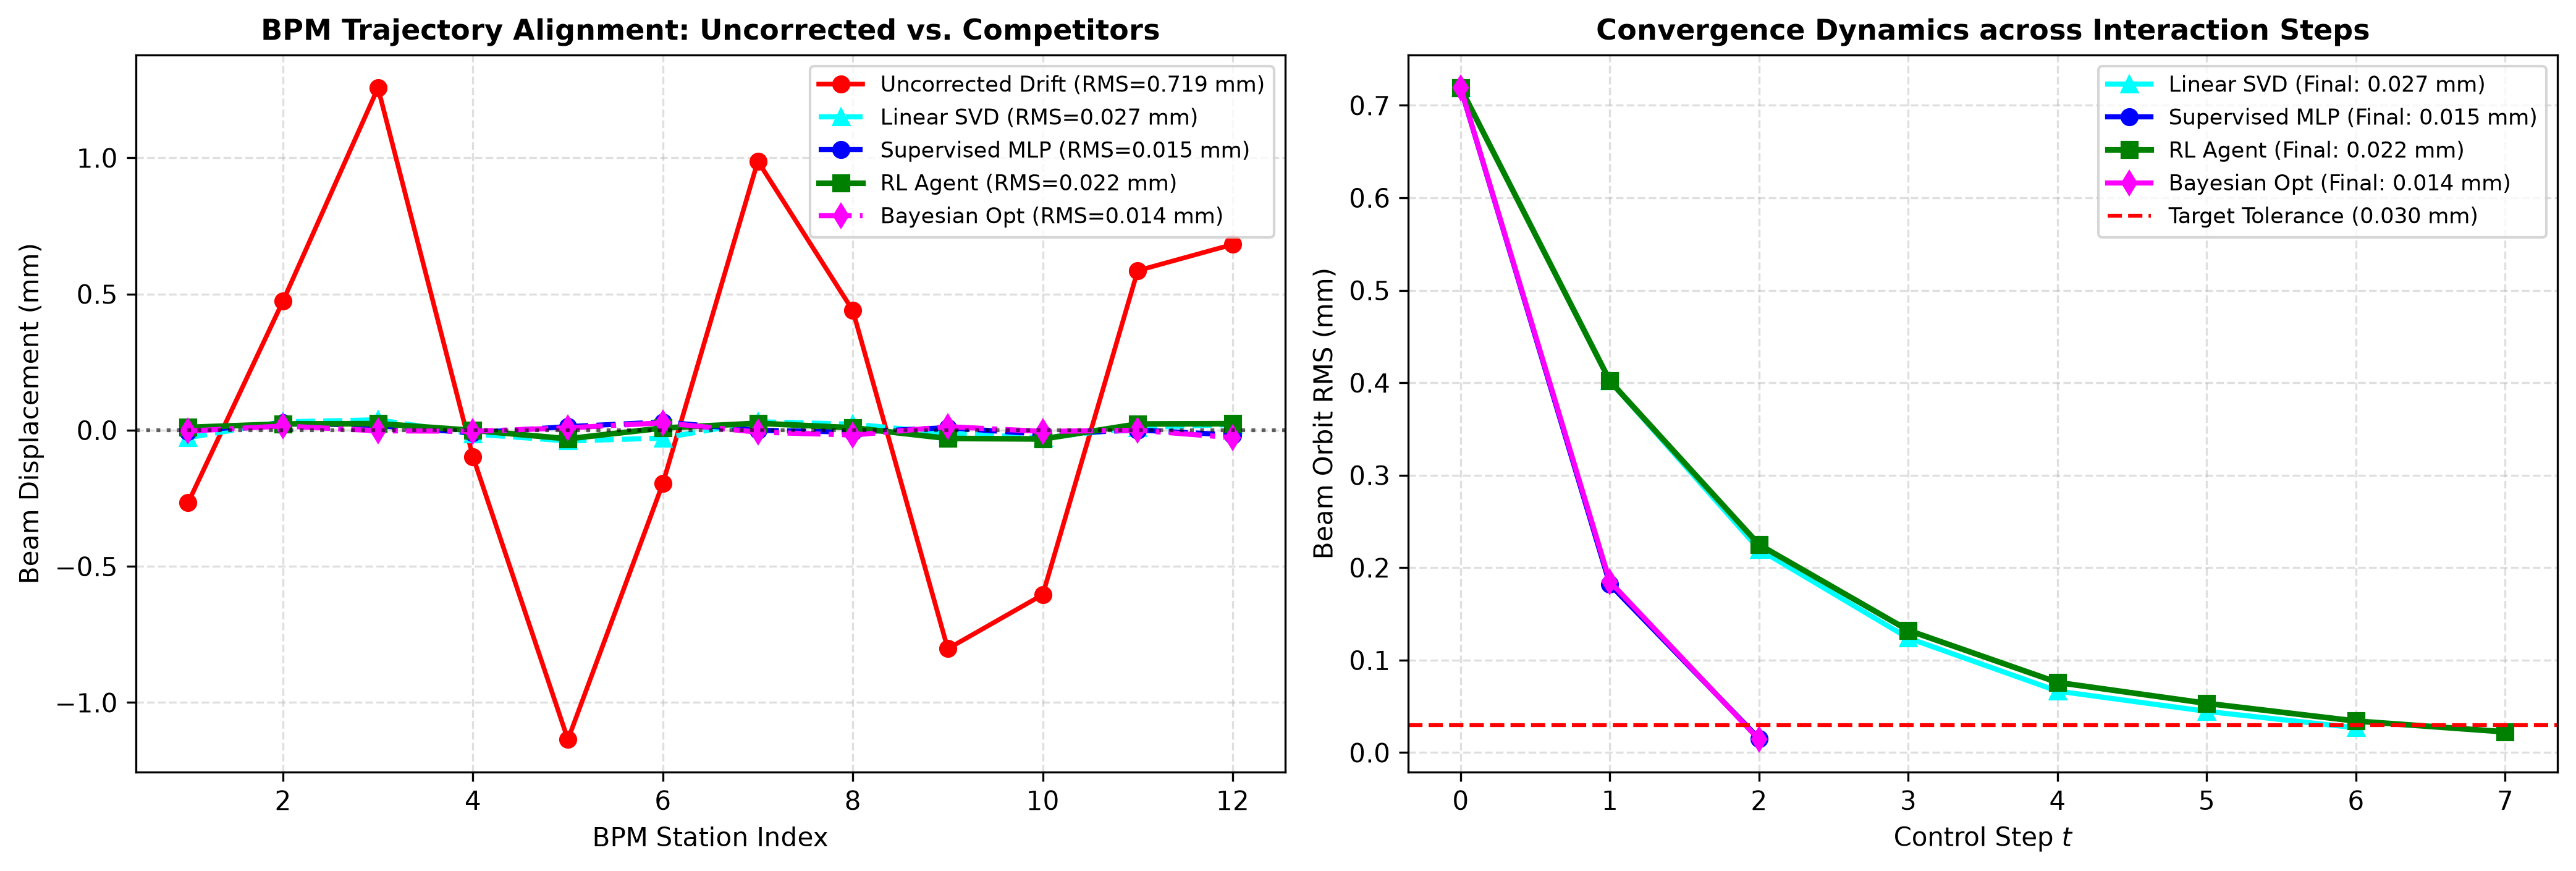
\includegraphics[width=8.6in,height=2.9in]{benchmark_trajectories.png}};

  % Clean Unwrapped Table at Top = 4.55in
  \node[anchor=north,inner sep=0pt]
    at ([yshift=-4.55in]current page.north) {%
      \renewcommand{\arraystretch}{1.22}
      \begin{tabular}{@{}llccccc@{}}
        \toprule
        \textbf{\color{primaryblue}Rank} & \textbf{\color{primaryblue}Controller Paradigm} & \textbf{\color{primaryblue}Success} & \textbf{\color{primaryblue}Mean Steps} & \textbf{\color{primaryblue}Final RMS} & \textbf{\color{primaryblue}Current} & \textbf{\color{primaryblue}Score} \\
        \midrule
        \textbf{\color{gold}Rank 1} & Track 3: Bayesian Optimization (BO) & \textbf{100.0\%} & \textbf{3.6 steps} & \textbf{0.0136 mm} & 3.85 A & \textbf{\color{gold}878.384 pts} \\
        \textbf{\color{primaryblue}Rank 2} & Baseline 1 (Track 1): Supervised Neural Inversion (MLP) & 100.0\% & 4.0 steps & 0.0197 mm & 3.84 A & \textbf{\color{primaryblue}779.169 pts} \\
        \textbf{Rank 3} & Baseline 0: Classical Linear SVD & 100.0\% & 9.4 steps & 0.0235 mm & 3.80 A & 635.277 pts \\
        \textbf{Rank 4} & Track 2: Closed-Loop RL Policy Agent & 100.0\% & 10.8 steps & 0.0256 mm & 3.79 A & 590.559 pts \\
        \bottomrule
      \end{tabular}
    };

  \slidefooter{32}
\end{tikzpicture}
\clearpage

% ==============================================================================
% SLIDE 33: Method Comparison Summary (Baselines & Tracks)
% ==============================================================================
\begin{tikzpicture}[remember picture,overlay]
  \slidespread{1.15}
  \slideheader{Evaluation Results}{Method Comparison Summary}{How the two baselines and the two challenge tracks differ, and how they score on the 30 seeds}

  \node[anchor=north,inner sep=0pt]
    at ([yshift=-1.55in]current page.north) {%
      \fs{12}{14}\color{darkgray}%
      \renewcommand{\arraystretch}{1.45}
      \begin{tabular}{@{}>{\raggedright\arraybackslash}p{2.05in}>{\raggedright\arraybackslash}p{2.35in}>{\raggedright\arraybackslash}p{1.75in}>{\raggedright\arraybackslash}p{1.95in}>{\raggedright\arraybackslash}p{2.1in}>{\centering\arraybackslash}p{1.45in}@{}}
        \toprule
        \textbf{\color{primaryblue}Method} & \textbf{\color{primaryblue}Control law} & \textbf{\color{primaryblue}Model \& data} & \textbf{\color{primaryblue}Strengths} & \textbf{\color{primaryblue}Limitations} & \textbf{\color{primaryblue}Score: ref.\ / solution} \\
        \midrule
        \textbf{\color{navy}Baseline 0}\newline Classical SVD & $\Delta\mathbf{I} = -\alpha(\mathbf{R}^T)^\dagger\mathbf{Y}$, fixed gain $\alpha = 0.45$ & Analytic ORM; no training data & Instant, robust, interpretable & Ignores saturation; slow at low gain; fixed reference & 635.277 / --- \\
        \textbf{\color{navy}Baseline 1 (Track 1)}\newline Supervised inversion & Minimize $\|\mathbf{Y} - f_\theta(\mathbf{I}) + f_\theta(\mathbf{I}+\Delta\mathbf{I})\|^2$ with L-BFGS-B each step & MLP digital twin; 1,500 offline shots & Learns the non-linear response & Only as good as the surrogate; about 27 ms per step & 779.169 / 924.2 \\
        \textbf{\color{navy}Track 2}\newline RL / adaptive policy & Physics prior $+$ learned residual $+$ damping & Policy parameters; tuned in closed loop & Fastest per step; adapts online & Gain and damping tuning; overshoot risk & 590.559 / 940.0 \\
        \textbf{\color{navy}Track 3}\newline Bayesian optimization & Minimize LCB of GP-predicted RMS each step & Gaussian process; $\sim$300 calibration shots & Sample-efficient; models uncertainty & GP cost grows with data; slowest per step (about 66 ms) & 878.384 / 909.9 \\
        \bottomrule
      \end{tabular}
    };

  \at{0.8}{5.95}{11.733}{\fs{10.5}{13.5}\color{mutedgray}%
    Reference: unmodified notebook controllers (per-seed 0--1000 scoring, mean over 30 seeds). Solution: the organizers' worked solution, which inverts the model on the total current. Baseline 0 is a fixed reference and is not tuned by participants.
  }

  \slidefooter{33}
\end{tikzpicture}
\clearpage

% ==============================================================================
% SLIDE 34: Strategic Advice for Competitors
% ==============================================================================
\begin{tikzpicture}[remember picture,overlay]
  \slidespread{1.39}
  \slideheader{Competitor Strategy}{Strategic Advice for Competitors}{Practical engineering guidance to maximize benchmark score and avoid common failure modes}

  \drawcard{0.8}{1.4}{11.733}{5.3}{Engineering Best Practices for Orbit Control}
  \at{1.1}{2.1}{11.1}{\fs{13.5}{19}\color{darkgray}%
    {\fs{15}{18}\bfseries\color{navy}1. If Your Controller Oscillates or Diverges Near Target:}\\[0.3em]
    $\bullet$ Check your feedback gain $\alpha$. With the plain pseudo-inverse, gains up to about $1.2$ converge fastest (3.7 steps at $1.2$ vs.\ 9.4 at $0.45$); above that the controller overshoots.\\
    $\bullet$ Compensate the cubic saturation on the total current from \texttt{info[\textquotedbl{}currents\textquotedbl{}]}: with gain $1.0$ this lands in about 3.7 steps at 924 points.\\
    $\bullet$ Step damping $\gamma(t) = 1.0 / (1.0 + \kappa \cdot t)$ is a trade-off: it helped at gain 1.0 and cost points at gains 0.45 and 1.2.\\[0.9em]
    {\fs{15}{18}\bfseries\color{navy}2. If Your Neural Surrogate Has High Generalization Error:}\\[0.3em]
    $\bullet$ Ensure your training dataset covers steerer excitations across $[-3.0, +3.0]\text{ A}$ so that non-linear cubic saturation is well-sampled.\\
    $\bullet$ Check the holdout RMSE: the default MLP stops at 0.109 mm. Try \texttt{activation='tanh'} with \texttt{solver='lbfgs'} (0.012 mm).\\[0.9em]
    {\fs{15}{18}\bfseries\color{navy}3. Real-Time Telemetry Logging:}\\[0.3em]
    $\bullet$ Connect your notebook runs to Weights \& Biases (\texttt{wandb.ai}) to visualize step-by-step RMS decay against reference baselines on the live leaderboard.
  }

  \slidefooter{34}
\end{tikzpicture}
\clearpage

% ==============================================================================
% SLIDE 35: Summary & Transition to Lecture 2
% ==============================================================================
\begin{tikzpicture}[remember picture,overlay]
  \slidespread{1.08}
  \slideheader{Conclusion \& Roadmap}{Summary \& Transition to Lecture 2}{Key conclusions from Lecture 1 and orientation for the upcoming agentic AI session}

  \drawcard{0.8}{1.4}{11.733}{5.3}{Key Takeaways \& What Comes Next}
  \at{1.1}{2.1}{11.1}{\fs{13.5}{19}\color{darkgray}%
    {\fs{15}{18}\bfseries\color{navy}Four Core Takeaways from Lecture 1:}\\[0.3em]
    \textbf{1. Physics Guides the AI:} The ORM pseudo-inverse works from the first step and reaches the target on all 30 seeds; learning supplies what the linear model lacks.\\
    \textbf{2. Total Current Matters:} Saturation depends on the total current. Controllers that model it gain about 100 points over the best plain pseudo-inverse (924 vs.\ 822).\\
    \textbf{3. Judge a Surrogate by its Holdout Error:} The reference MLP (0.109 mm) is worse than a linear model (0.082 mm); a well-trained one reaches 0.012 mm.\\
    \textbf{4. Respect the Limits:} The 0.8 A step limit sets a floor of 3 to 4 steps; the $10\ \mu\text{m}$ noise sets the precision floor. A GP on 300 shots leads the references (878).\\[1.0em]
    {\fs{15}{18}\bfseries\color{navy}Next Session (10:40 -- 12:00):}\\[0.3em]
    {\fs{16}{20}\bfseries\color{primaryblue}Lecture 2: Agentic AI for Accelerator Research (Osprey Applications)}\\[0.2em]
    \textbf{Speaker:} Thorsten Hellert, Ph.D. (Lawrence Berkeley National Laboratory)\\
    \textbf{Topic:} Autonomous operational agents, dynamic tool calling, and automated scientific workflows.\\[1.0em]
    {\fs{16}{20}\bfseries\color{accent}Q \& A Discussion}
  }

  \slidefooter{35}
\end{tikzpicture}

\end{document}
